\documentclass{article}
\usepackage[utf8]{inputenc}
\usepackage{graphicx}
\usepackage[a4paper, total={8in, 10.5in}]{geometry}
\usepackage{rotating}
\usepackage{afterpage}
\usepackage{url}

\usepackage{algorithm}
\usepackage{algpseudocode}
\usepackage{amsmath}
\usepackage{mathtools}
\usepackage{tabularx}
\usepackage{caption}
\usepackage{subcaption}
\usepackage{afterpage}
\usepackage{titlepic}
\usepackage{gensymb}
\usepackage{float}
\usepackage{hyperref}


\title{%
  A Numerical Analysis of Convection in the Inner Core \\
  \large Third Year Physics ASC  \\
    Start Date: 16th of August 2021 End Date: 29th of October 2021}

\author{Maximilian Williams (u6338634)}
\titlepic{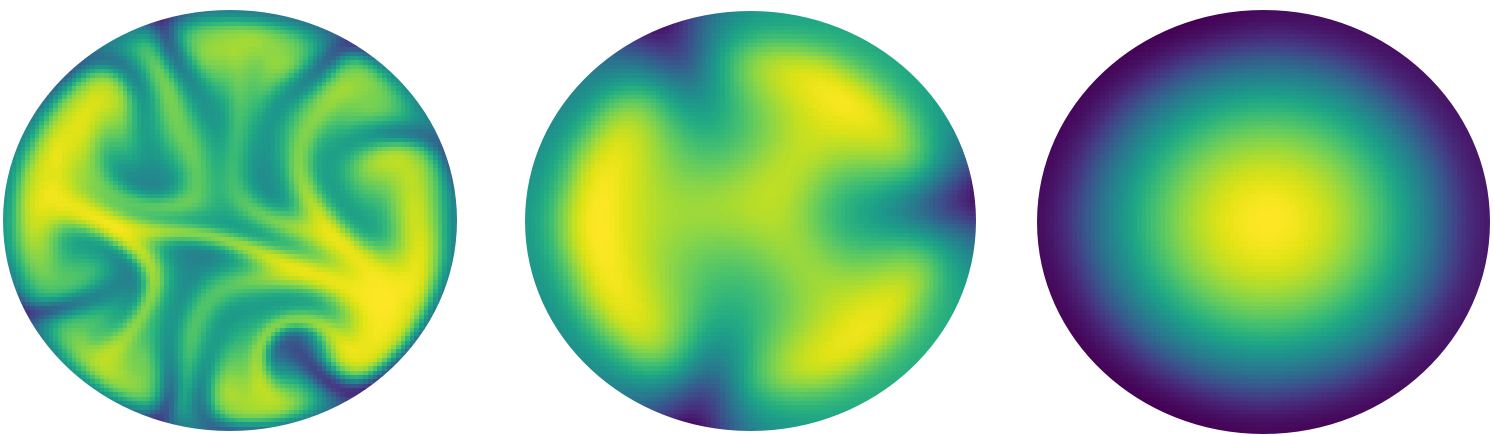
\includegraphics[width=\textwidth]{introfigure.png}}
\date{October 2021}

\begin{document}

\maketitle

\begin{abstract}

	\noindent Whether The Earth's inner core convects or not has been a contentious topic 
	in geoscience. Here we numerically model the Earth's inner core as a self-gravitating 
	internally heated fluid 
	in 2-dimensions using a streamfunction-vorticity method and a Thermal Lattice Boltzmann 
	approach coded from scratch in Python3 and goLang. By 
	comparing results of two simple 
	streamfunction-vorticity codes we conclude that the polar geometry of our 2-dimensional
	inner core model and the central region are important in 
	modelling convection. Using a Thermal Lattice Boltzmann method (TLBM) we simulate the 
	entire domain while respecting the geometry. Our TLBM simulations are in the high 
	Prandtl number limit with $Pr=5000$ and give an upper bound on the critical internally 
	heated Rayleigh number of $Ra_H = 10^5$. 
 
\end{abstract}

\section*{Introduction}
The Earth's inner core is a particularly interesting subterranean region as it helps maintain Earth's magnetic field which shields life on Earth from
solar 
radiation. Yet this critical region of the Earth is relatively poorly understood. It sits within the liquid outer core, which shares a boundary with a sharp 
density change with the lower mantle and is opaque to S-waves \cite{fowler1990solid}. This makes seismic signals which pass through the inner core such 
as PKJKP and PKIKP waves difficult to detect \cite{tkalvcic2018shear, bolt1970pdp}. The inner core is also one of the most extreme environments, with 
temperatures exceeding $5000^{\circ}$C and pressures exceeding 3 million atmospheres which are 
largely outside of experimental material physics, making composition and physical properties difficult to obtain. Ignoring these difficulties, modelling 
convection in the inner core is also non-trivial due to internal heating and non constant gravity. Emulating varying gravitation and internal heating 
directly in experiment is difficult. For this reason, the problem of convection in the inner core is well suited to numerical methods. 
\newline
\noindent In this report, a simplified model of the inner core and accompanying theory is presented. Two numerical methods for simulating this model, the streamfunction-vorticity method and Thermal Lattice Boltzmann method (TLBM) are introduced
and their implementations described. An advection test is performed on the streamfunction-vorticity code while a full convection simulation comparison is done between the TLBM 
implemented here and other work \cite{mora2017simulation}. Results from the streamfunction-vorticity code are presented showing the central region and geometry of the inner core model are important.
Finally, the TLBM code is used to produce high Prandtl number simulations with varying internally heated Rayleigh number to determine an upper bound on the critical Rayleigh number
for the model. The report concludes with a discussion of difficulties in using each technique, possible improvements and extensions for future work.
\vspace{0.3cm}
\newline
\noindent All codes produced for this report are available \href{https://github.com/maxzwilliams/ASC2021}{here} or at the url: \url{https://github.com/maxzwilliams/ASC2021}


%% I want to have a brief discussion of what I will do in this report.


\newpage
\subsection*{Physical Picture}
{\it{Here I talk about what I am modelling and my assumptions about the inner core.}}
\vspace{0.3cm}
\newline
Throughout this report, we approximate the Earth's inner core as a perfect liquid sphere and model a 
2-dimensional cross-section. We take the inner core as being internally heated except for a thin 
outer layer that is cooled. We ignore all affects of rotation or precession, assuming the core is 
in an inertial reference frame. We assume that the earth above the inner core is spherically 
symmetric in all respects and so model no variations in pressure or gravitation across the inner 
core's surface.
\newline
To simulate this model, we investigate two geometries. The first is a polar geometry shown in figure \ref{unrolling} (top) and is a more accurate depiction of the model. The second, is a Cartesian depiction of the model (figure \ref{unrolling} (bottom)) which is easier to simulate, but does not respect the geometry. It can be thought of as cutting the polar model at the $0,2\pi$ azimuthal boundary and stretching it out. 

\begin{figure}[H]
	\centering
	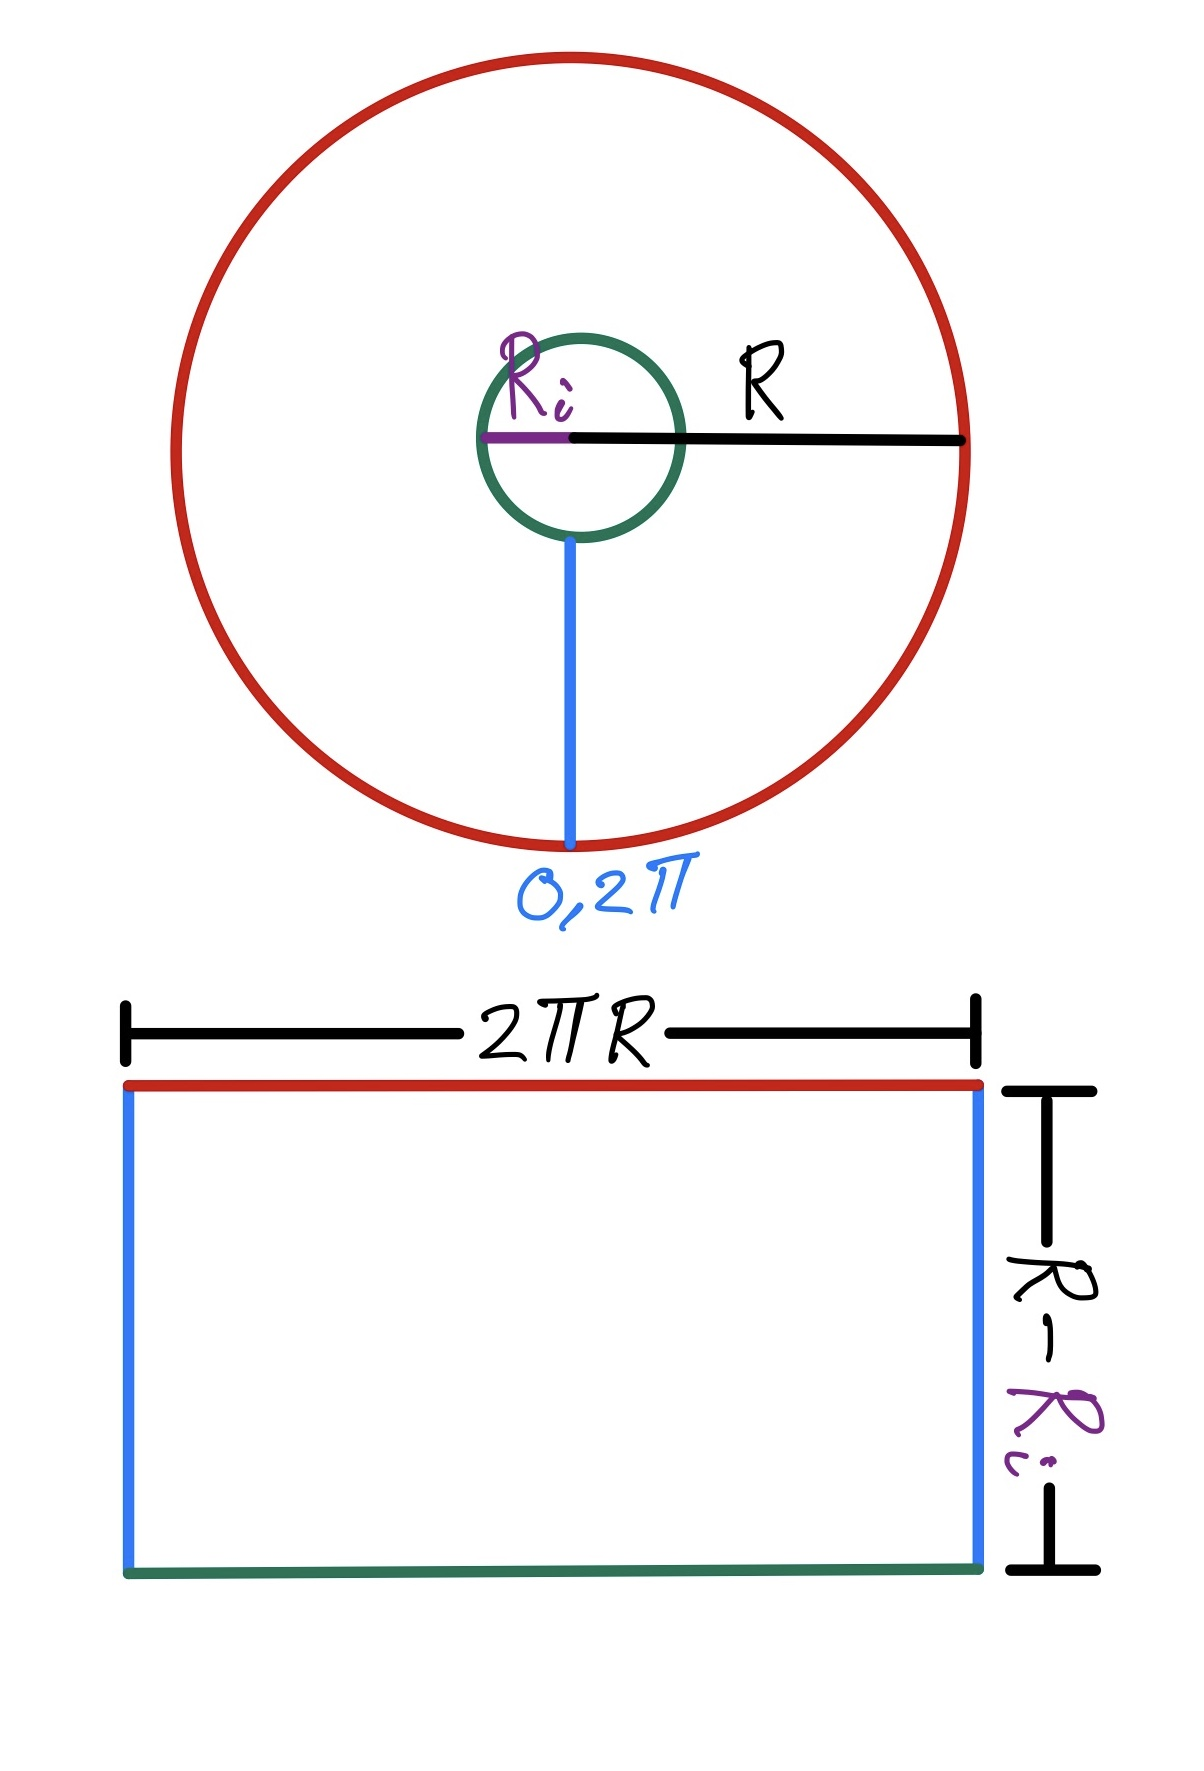
\includegraphics[scale=0.25]{unrap image.jpg}
	\caption{Figure showing how the 2-dimensional polar domain (top) is cut at the azimuthal angle $0, 2\pi$ boundary and stretched into the Cartesian geometry (bottom). Sides are color coded. $R$ and $R_i$ are the outer and inner radii of the polar domain.} 
	\label{unrolling}
\end{figure}



\subsection*{Governing Equations}
{\it{In this section I introduce the physics of the problem; the governing equations that we wish to numerically solve.}}
\vspace{0.3cm}
\newline
\noindent We describe the fluid in the inner core in the Eulerian frame under a graviational acceleration $\vec{g}$ which varies in space. We give 
each location in the fluid a time and space dependent velocity $\vec{u}$ and density $\rho$. We assume that the fluid is incompressible and its viscosity $\
mu$ and thermal diffusivity $\kappa$ are constant. By conserving fluid momentum, we produce the Navier-Stokes equation:
\begin{equation}
	\rho \frac{D \vec{u}}{D t} = \rho \vec{g} - \nabla p + \mu \nabla^2 \vec{u},
	\label{NSE}
\end{equation}
where $\frac{D}{D t} = \frac{\partial }{\partial t} + (\vec{u} \cdot \nabla)$ is the material derivative, $p$ the pressure and $\nabla$ the del 
operator. The dynamics of fluid temperature $T$ are described the the inhomogenous advection diffusion equation:
\begin{equation}
	\frac{D T}{D t} = \kappa \nabla^2 T + H,
	\label{adeT}
\end{equation}
where $H$ is internal heating \cite{goluskin2016internally}. The density of the fluid $\rho$ is assumed to vary linearly in temperature according to the equation of state:
\begin{equation}
	\rho = \rho_0 (1- \alpha(T - T_0)),
	\label{equation of state}
\end{equation}
where $\alpha$ is the volumetric expansion coefficient and $\rho_0$ the density at a reference temperature $T_0$. We assume the density variations are 
small and that the inner core is evolving on geologic timescales, allowing us to take the velocities $\vec{u}$ to be first order. These assumptions give 
the slow flow Boussinesq approximation \cite{goluskin2016internally, tritton2012physical} to equation \ref{NSE}:
\begin{equation}
	\frac{\partial \vec{u}}{\partial t} = \frac{\rho'}{\rho} \vec{g} -   \frac{\nabla p'}{\rho_0} + \nu \nabla^2 \vec{u},
	\label{NSE slow + boussinesq}
\end{equation}
where $\rho'=-\alpha(T - T_0)$, $\nu$ the kinematic viscosity $\nu = \frac{\mu}{\rho_0}$ and $p'$ a first order perturbation to the background pressure $
p_0$. 
\newline
\begin{equation}
	Pr = \frac{\nu}{\kappa}
	\label{prantl}
\end{equation}
We use two numbers to characterise the problem, the Prandtl number and the Rayleigh number \cite{goluskin2016internally}. The Prandtl number $Pr$ (equation \ref{prantl}) is the ratio 
of momentum and thermal diffusivity. We also use the Rayleigh number $Ra$ (equation \ref{Rayleigh number}):
\begin{equation}
	Ra = \frac{g \alpha \Delta T  d^3}{\nu \kappa},
	\label{Rayleigh number}
\end{equation}
where $\Delta T$ is the variation over the length scale of the problem $d$. The Rayleigh number is the ratio of timescales for thermal diffusion and 
thermal convection. High Rayleigh numbers $>\approx 650$ imply thermal convection. For internally heated problems such as ours, the temperature 
variation is poorly defined and so we use $\Delta T = \frac{H d^2}{\kappa}$ instead, giving the internally heated Rayleigh number \cite{goluskin2016internally}:
\begin{equation}
	Ra_{H} = \frac{g \alpha H d^5}{\nu {\kappa}^2}.
	\label{internally heated rayleigh number}
\end{equation}

\section*{Numerical Methods}
{\it{Two numerical methods are introduced for solving the thermal convection problem, the Lattice Boltzmann Method and the streamfunction-vorticity formulation.}}

\subsection*{Streamfunction-Vorticity formulation}
{\it{Here I introduce the streamfunction-vorticity method for use in 2 dimensions and use it to eliminate pressure terms in \ref{NSE slow + boussinesq} and \ref{adeT} in Cartesian and polar geometries giving a set of numerically solvable equations.}}
\vspace{0.3cm}
\newline
\noindent The streamfunction-vorticity formulation is a popular method for analytical 
and simple numerical analysis of incompressible fluids in two dimensions. Its main 
advantage is its elimination of all pressure terms, which would typically require 
iterative techniques to solve, an example being the SIMPLE algorithm and its derivatives 
\cite{earn2017investigation}. However, the streamfunction-vorticity method is limited to 
2-dimensional and 3-dimensional symmetric flows and so has limited applications.
\newline

\noindent We define a direction $\hat{z}$ out of the plane of our inner core model. We define scalar vorticity $\omega$ by:
\begin{equation}
	\omega = (\nabla \times \vec{u})_z,
	\label{omega}
\end{equation}
where the $z$ subscript $z$ is out of the simulation plane, and scalar streamfunction $\psi$ implicitly by:
\begin{equation}
	\omega = - \nabla^2 \psi.
	\label{psi}
\end{equation}
Given a coordinate system, and a clever definition of velocities $\vec{u}$ we can rewrite equations \ref{adeT} and \ref{NSE slow + boussinesq} in terms of $\omega$ and $\psi$ rather than $\vec{u}$ and $p$ \cite{tritton2012physical}. In Cartesian coordinates $(x,y)$ with $\vec{u} = u \hat{x} + v \hat{y}$ we pick 
\begin{equation}
	u = \frac{\partial \psi}{\partial y}, v = -\frac{\partial \psi}{\partial x},
	\label{cartesian velocities}
\end{equation}
allowing us to write equations \ref{adeT} and \ref{NSE slow + boussinesq} as:
\begin{tabularx}{\textwidth}{XX}
\begin{equation}
	\frac{\partial T}{\partial t} + \frac{\partial \psi}{\partial y} \frac{\partial T}{\partial x} - \frac{\partial \psi}{\partial x} \frac{\partial T}{\partial y} = \kappa \nabla^2 T + H
	\label{adeT sfvt cartesian}
\end{equation}
    &
\begin{equation}
	\frac{\partial \omega}{\partial t} = -\frac{g_y}{\rho_0} \frac{\partial \rho'}{\partial x} + \nu \nabla^2 \omega
	\label{NSE slow + boussinesq sfvt cartesian}
\end{equation}
\end{tabularx}\par
\noindent Similarly, in polar coordinates (r, $\theta$) with $\vec{u} = u \hat{r} + v \hat{\theta}$ we pick:
\begin{equation}
	u = \frac{1}{r} \frac{\partial \psi}{\partial \theta}, v = -\frac{\partial \psi}{\partial r},
	\label{polar velocities}
\end{equation}
giving:
\begin{tabularx}{\textwidth}{XX}
\begin{equation}
	\frac{\partial T}{\partial t} + \frac{1}{r} \frac{\partial \psi}{\partial \theta} \frac{\partial T}{\partial r} - \frac{1}{r} \frac{\partial \psi}{\partial r} \frac{\partial T}{\partial \theta} = \kappa \nabla^2 T + H
	\label{adeT sfvt polar}
\end{equation}
    &
\begin{equation}
	\frac{\partial \omega}{\partial t} = - \frac{g_r}{\rho_0 r} \frac{\partial \rho'}{\partial \theta} +\nu \nabla^2 \omega.
	\label{NSE slow + boussinesq sfvt polar}
\end{equation}
\end{tabularx}\par
\noindent Importantly, our definitions of $u$ and $v$ in equations \ref{cartesian velocities} and \ref{polar velocities} satisfy equation \ref{omega} and \ref{psi}. Equations \ref{psi}, \ref{adeT sfvt cartesian}, \ref{NSE slow + boussinesq sfvt cartesian} for the Cartesian case and \ref{psi}, \ref{adeT sfvt polar}, \ref{NSE slow + boussinesq sfvt polar} for the polar case can be directly solved.

\subsubsection*{Solving the Streamfunction-Vorticity equations}
{\it{The finite difference method used to solve the streamfunction-vorticity-formulated governing equations in my streamfunction-vorticity codes for Cartesian and polar geometries is described. }}
\vspace{0.3cm}
\newline
\noindent We first discretize our domain $\mathcal{D}$. In the Cartesian case, we use $(x_i,y_j)=(i \Delta x, j \Delta y)
$ with integers $i$ and $j$ satisfying $0\leq i < N_x$ $0 \leq j < N_y$. In the polar case, we use $(r_i, \theta_j)= (R_0 
+ i \Delta r, j 
\Delta \theta)$ again with  $0 \leq i < N_r$ and $0 \leq j < N_{\theta}$. We impose $\Delta \theta = \frac{2 \pi}
{N_{\theta} - 1}$ for consistency with $\theta$-periodic boundary conditions and an inner radius $R_0$ in polar 
coordinates to avoid 
singularities at $r=0$. This inability to model the innermost region is an important deficiency of the streamfunction-vorticity method in polar coordinates. We discretize time $t$ by $t_n = n \Delta t$. For a function $f$, we use 
$f^n_{i,j}$ to denote $f$ evaluated at time $n$ at position $(x_i,y_j)$ in Cartesian coordinates or $(r_i, \theta_j)$ in 
polar coordinates. 
\newline
To approximate derivatives we use a finite difference approach. All time derivatives are approximated by forward difference \cite{press1986numerical}:
\begin{equation}
	\frac{\partial f}{\partial t} = \frac{f^{n+1} - f^{n}}{\Delta t}
	\label{forward time difference}
\end{equation}
Second order space derivatives are approximated by a central difference \cite{press1986numerical}:

\begin{tabularx}{\textwidth}{XX}
\begin{equation}
	\frac{\partial^2 f_{i,j}}{\partial {x_1}^2} = \frac{f_{i+1,j} - 2 f_{i,j} + f_{i-1,j}}{{\Delta x_1}^2},
\end{equation}
    &
\begin{equation}
	\frac{\partial^2 f_{i,j}}{\partial {x_2}^2} = \frac{f_{i,j+1} - 2 f_{i,j} + f_{i,j-1}}{{\Delta x_2}^2},
\end{equation}
\end{tabularx}
where $x_1$ is the first coordinate and $x_2$ is the second coordinate. For example, in Cartesian coordinates $(x,y)$, we would have $x_1=x$ and $x_2=y$. 
For non advection terms, we approximate first order spatial derivatives by \cite{press1986numerical}:
\begin{equation}
	\frac{\partial f_{i,j}}{\partial x_1} = \frac{f_{i+1,j} - f_{i-1,j}}{2{\Delta x_1}},
\end{equation}
and
\begin{equation}
	\frac{\partial f_{i,j}}{\partial x_2} = \frac{f_{i,j+1} - f_{i,j+1}}{2{\Delta x_2}}.
\end{equation}
For advection terms, of the form $a \frac{\partial f_{i,j}}{\partial x_1}$ we employ a first order Godunov scheme \cite{godunov1959difference, guinot2003godunov}:
\begin{equation}
	a \frac{\partial f_{i,j}}{\partial x_1} = \frac{1}{\Delta x} ( \mid a\mid (  \frac{1}{2} f_{i+1,j} - \frac{1}{2} f_{i-1,j}   ) - a ( \frac{1}{2} f_{i+1,j} -f_{i,j} - \frac{1}{2} f_{i-1,j} )).
\end{equation}
This scheme is always upstream, regardless of the direction of the advecting field $a$ and is stable so long as $\mid a \mid \frac{\Delta t}{\Delta x} \leq 1$. Using this Godunov scheme, the modified equivalent partial differential equation for the advection diffusion equation shows a numerical diffusion with constant $\kappa' = \mid a \mid \frac{\Delta x}{2} (1 - \mid a \mid \frac{\Delta t}{\Delta x})$ which can be made small relative to the diffusion constant $\kappa$ by taking a fine mesh ($\Delta x \rightarrow 0$). 
\newline
A lot of time in this project was spent getting a stable and accurate advection scheme. Simple schemes for advection were tried such as Lax-Wendroff, central difference and forwards/backwards Euler. These schemes either introduced large numerical diffusion or were unconditionally unstable. Other more accurate, but substantially more complex methods for solving these equations, particularly the advection equation exists such as the Semi-Lagrange Crank-Nicholson scheme \cite{spiegelman2006semi}.
\newline
To solve the streamfunction-vorticity equations we assume a starting vorticity $\omega$ on our domain $\mathcal{D}$. We then apply the Jacobi method (given in appendix) to solve equation \ref{psi} for $\psi$ on the interior of the domain which we call $\mathcal{D}'$. 
Using $\psi$ we update $T$ on $\mathcal{D}'$ using equation \ref{adeT sfvt cartesian} (or \ref{adeT sfvt polar} for polar). Finally, $\omega$ is updated on $\mathcal{D}'$ using 
equation \ref{NSE slow + boussinesq sfvt cartesian} (\ref{NSE slow + boussinesq sfvt polar} for polar) \cite{adair2015developing}. This process is repeated.
\newline
Using this streamfunction-vorticity method we simulate the polar (figure \ref{unrolling} (top)) and Cartesian (figure \ref{unrolling}) model. Critically, the polar simulation does not include the innermost region.




\subsection*{Lattice Boltzmann Method}
{\it{In this section I give a brief introduction to the Lattice Boltzmann Method and why its different from traditional techniques. I introduce a 2-dimensional lattice D2Q9 and describe the Thermal Lattice Boltzmann method (TLBM) which is employed by my code to simulate convection. I then show how the Lattice Boltzmann method can be used to simulate the polar model while still maintaining the inner region which the streamfunction-vorticity polar model lacks.}}
\vspace{0.3cm}
\newline
\noindent The Lattice Boltzmann Method (LBM) is a generalization of a Lattice Gas Automata (LGA) , which are themselves a 
specialized Automata for simulating fluid flows \cite{rothman2004lattice}. These Automata methods like common fluid simulation techniques 
discretize space and time. They directly simulate the state of particles or their distributions and evolve in time 
according to simple rules which give the desired macroscopic fluid properties as an emergent effect \cite{wagner2008practical}. This is fundamentally 
different to typical approaches which amount to directly numerically solving a set of partial differential equations. In the Thermal Lattice Boltzmann method (TLBM) the internal energy is also simulated and used to simulate thermal affects which couple to the motion of the particles.
\newline
\noindent To discretize space, we place nodes at locations $(x_i,y_j)=(i,j)$ with $i,j$ integers. Each node has attached to it a lattice, here the D2Q9 lattice shown in figure \ref{D2Q9}. The lattice defines unit vectors $\vec{e}_i$, $i \in \{ 0,1,2,3,4,5,6,7,8 \}$ \cite{mora2017simulation}. In addition, each direction $e_i$ gets a weight $w_i$ \cite{mora2017simulation}. In the D2Q9 lattice these are:
\begin{equation*}
w_i = \begin{cases}
          \frac{4}{9} \quad &\text{if}  \ i=0 \\
          \frac{1}{9} \quad &\text{if} \ i=1,2,3,4 \\
          \frac{1}{36} \quad &\text{if} \ i=5,6,7,8 \\
     \end{cases}.
\end{equation*}
\begin{figure}[H]
	\centering
	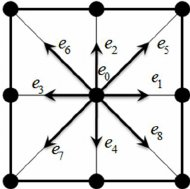
\includegraphics{D2Q9Lattice.jpg}
	\caption{D2Q9 Lattice. Black nodes represent lattice points, vectors $e_0,..,e_8$ are the lattice vectors. Image sourced from \cite{khazaeli2015ghost}}
	\label{D2Q9}
\end{figure}
\noindent We wish to simulate convection. For this, we require the particle motion and the internal energy throughout the lattice. We define two distribution functions $f_{\alpha}(\vec{x}, t)$ and $g_{\alpha}(\vec{x}, t)$ denoting the particle and internal energy distributions along direction $\alpha$ at lattice points $\vec{x}$ and times $t$. The direction can be thought of as the direction of flow for particles or energy. Each timestep there are two steps to updating $f$ and $g$, a streaming step:
\newline
\begin{tabularx}{\textwidth}{XX}
\begin{equation}
	f_{\alpha}(\vec{x} + \vec{e}_\alpha, t + \Delta t) = f_{\alpha}(\vec{x}, t),
	\label{streaming step}
\end{equation}
    &
\begin{equation}
	g_{\alpha}(\vec{x} + \vec{e}_\alpha, t + \Delta t) = g_{\alpha}(\vec{x}, t),
\end{equation}
\end{tabularx}\par
\noindent and a collision step:
\newline
\begin{tabularx}{\textwidth}{XX}
\begin{equation}
	f_{\alpha}(\vec{x} + \vec{e}_{\alpha}, t + \Delta t) = f_{\alpha}(\vec{x}, t) + \frac{1}{\tau_f} (f^{eq}_{\alpha}(\vec{x}, t)  - f_{\alpha}(\vec{x}, t)) + F_{\alpha}
	\label{f collision step}
\end{equation}
    &
\begin{equation}
	g_{\alpha}(\vec{x} + \vec{e}_{\alpha}, t + \Delta t) = g_{\alpha}(\vec{x}, t) + \frac{1}{\tau_g} (g^{eq}_{\alpha}(\vec{x}, t)  - g_{\alpha}(\vec{x}, t)) + G_{\alpha}.
	\label{g collision step}
\end{equation}
\end{tabularx}\par
\noindent Here $F_{\alpha}$ and $G_{\alpha}$ are the forcing terms terms and $f^{eq}_{\alpha}$ and $g^{eq}_{\alpha}$ are equilibrium distributions. The relaxation times $\tau_f$ and $\tau_g$ are related to the macroscopic thermal diffusivity ($\kappa$) and kinematic viscosity $\nu$ by \cite{mora2017simulation}:
\newline
\begin{tabularx}{\textwidth}{XX}
\begin{equation}
	\tau_g = \frac{3 \kappa}{S^2 \Delta t} + \frac{1}{2},
\end{equation}
    &
\begin{equation}
	\tau_f = \frac{3 \nu}{S^2 \Delta t} + \frac{1}{2}.
\end{equation}
\end{tabularx}\par
\noindent The equilibrium distributions are given by the BGK approximation \cite{qian1992lattice, rothman2004lattice}:
\newline
\begin{tabularx}{\textwidth}{XX}
\begin{equation}
	f^{eq}_{\alpha}(\vec{x}, t)  = \rho w_{\alpha} (1 + 3 \frac{\vec{e}_{\alpha} \cdot \vec{u}}{s^2} + \frac{9}{2} \frac{(\vec{e}_{\alpha} \cdot \vec{u}  )^2}{c^4} - \frac{3}{2} \frac{\vec{u} \cdot \vec{u}}{c^2}  ),
\end{equation}
    &
\begin{equation}
	g^{eq}_{\alpha}(\vec{x}, t)  = \epsilon \rho w_{\alpha} (1 + 3 \frac{\vec{e}_{\alpha} \cdot \vec{u}}{s^2} + \frac{9}{2} \frac{(\vec{e}_{\alpha} \cdot \vec{u}  )^2}{c^4} - \frac{3}{2} \frac{\vec{u} \cdot \vec{u}}{c^2}  )
\end{equation}
\end{tabularx}\par

\noindent Here $\rho$, $\epsilon$ and $\vec{u}$ are the macroscopic density, internal energy and velocity given by \cite{mora2017simulation}:

\begin{tabularx}{\textwidth}{XXX}
\begin{equation}
	\rho = \sum_{i=0}^{8} f_{i},
	\label{LBM rho}
\end{equation}
    &
\begin{equation}
	\rho \vec{u} = \sum_{i=0}^{i=8} f_{i} \vec{e}_{i}
	\label{LBM u}
\end{equation}
	&
\begin{equation}
	\rho \epsilon = \sum_{i=0}^{i=8} g_{i}.
	\label{LBM ep}
\end{equation}
\end{tabularx}\par

\noindent The forcing terms $F_i$ and $G_i$ are problem dependent. For thermal convection 
$G_i=0$ and $F_i$ is a gravitational term ${\Delta f}_{\alpha}$ \cite{mora2017simulation}:
\begin{equation}
	{\Delta f}_{\alpha} = - 
	\frac{w_{\alpha} \rho \alpha \epsilon}{\tau_{grav}}
	 \frac{\vec{e}_{\alpha}}{\mid \vec{e}_{\alpha} \mid} \cdot \vec{g} ,
\end{equation}
\noindent where $\mid \cdot \mid$ is the vector norm and $\vec{g}$ is the gravitational 
acceleration. Here $\tau_{grav}$ is the relaxation time for the gravitational field. We 
take $\tau_g=0.6$ here, following \cite{mora2017simulation}. The algorithm used to evolve 
the above TLBM equations is given in algorithm \ref{alg:TLBM} and closely follows 
\cite{mora2017simulation}.
\newline
%% Here I want to explain how I simulate my model in the Lattice Boltzmann method.
\noindent To simulate our model using the Lattice Boltzmann method, we define a Cartesian domain in which we place a circular boundary. We view this internal circular region as our model, and simulate gravity, internal heating/cooling and our fluid within it. This is seen in figure \ref{TLBM model}. This is possible only due to the ease of setting boundary conditions in the TLBM and can not easily be done in the streamfunction-formulation.
Critically, this simulation respects the polar geometry of our model while simulating its central region, which neither the polar or Cartesian streamfunction-vorticity simulations do simultaneously.

\begin{figure}[H]
	\centering
	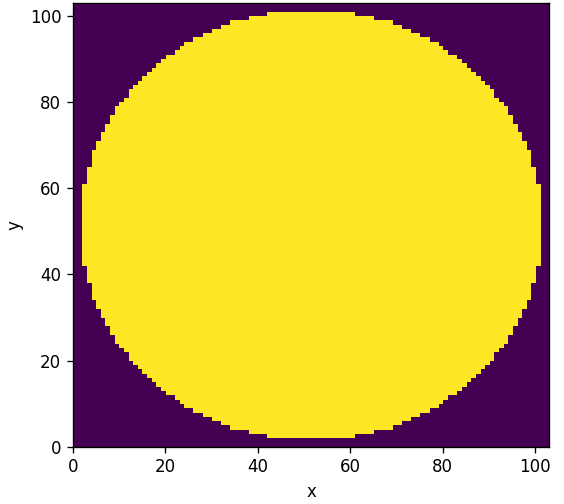
\includegraphics{latticeBoltzmanModel.png}
	\caption{Lattice Boltzmann code simulated on a Cartesian domain with circular boundary. Inside the circular region (yellow) the fluid is simulated while the exterior (purple) contains nothing and is not relevant to the simulation.}
	\label{TLBM model}
\end{figure}






\begin{algorithm}[h!]
\caption{Thermal Lattice Boltzmann Algorithm}\label{alg:TLBM}
\begin{algorithmic}

\State $f_{\alpha} = \rho_0 w_{\alpha}$ \Comment{Set particle distribution in domain}
\State $g_{\alpha} = 0$ \Comment{Set internal energy zero in domain}
\State $\epsilon = 0$ \Comment{Allocate memory for internal energy}
\State $\epsilon_b$ \Comment{Set heat field in the domain}
\State $\rho = 0$ \Comment{Allocate memory for density}
\State $\vec{u} = 0$ \Comment{Allocate memory for velocities}
\While{Simulation Running} \Comment{Begin main simulation loop}
	\State $g_{\alpha} \mathrel{+}= \rho \epsilon_b w_{\alpha} $ \Comment{At each timestep, add the affect of the heating field}
	\If{$x-\vec{e}_{\alpha}$ is solid} \Comment{The following 3 lines enforce bounce-back boundary conditions}
		\State $f_{\alpha}(x) = f_{\alpha'}(x)$
		\State $g_{\alpha}(x) = g_{\alpha'}(x)$
	\Else
		\State $f_{\alpha}(x) = f_{\alpha}(x - \vec{e}_{\alpha})$ \Comment{Streaming step}
		\State $g_{\alpha}(x) = g_{\alpha}(x - \vec{e}_{\alpha})$
	\EndIf
	\State $\rho = \sum_{i=0}^{i=8} f_{i}$ \Comment{Compute and set macroscopic density}
	\State $\vec{u} =\frac{(\sum_{i=0}^{i=8} f_{i} \vec{e}_{i})}{\rho} $ \Comment{Compute and set  macroscopic velocity}
	\State $\epsilon = \frac{\sum_{i=0}^{i=8} g_{i}}{\rho}$ \Comment{Compute and set internal energy}
	\State $f^{eq}_{\alpha} = \rho w_{\alpha} (1 + 3 \frac{\vec{e}_{\alpha} \cdot \vec{u}}{s^2} + \frac{9}{2} \frac{(\vec{e}_{\alpha} \cdot \vec{u}  )^2}{c^4} - \frac{3}{2} \frac{\vec{u} \cdot \vec{u}}{c^2})  $ \Comment{Get equilibrium distribution f}
	\State $g^{eq}_{\alpha}(\vec{x}, t)  = \epsilon \rho w_{\alpha} (1 + 3 \frac{\vec{e}_{\alpha} \cdot \vec{u}}{s^2} + \frac{9}{2} \frac{(\vec{e}_{\alpha} \cdot \vec{u}  )^2}{c^4} - \frac{3}{2} \frac{\vec{u} \cdot \vec{u}}{c^2}  ) $ \Comment{Get equilibrium distribution g}
	\State ${\Delta f}_{\alpha} = - w_{\alpha} \rho \alpha \epsilon \frac{\vec{e}_{\alpha}}{\mid \vec{e}_{\alpha} \mid} \cdot \vec{g}$ \Comment{Get gravitational term}
	\State $\tau_g = \frac{3 \kappa}{S^2 \Delta t} + \frac{1}{2}$ \Comment{Compute relaxation times}
	\State $\tau_f = \frac{3 \nu}{S^2 \Delta t} + \frac{1}{2}$
	\State $f_{\alpha} = f_{\alpha} + \frac{f^{eq}_{\alpha}-f_{\alpha}}{\tau_f} + {\Delta f}_{\alpha}$ \Comment{Collision step}
	\State $g_{\alpha} = g_{\alpha} + \frac{g^{eq}_{\alpha}-g_{\alpha}}{\tau_g}$
\EndWhile
\end{algorithmic}
\end{algorithm}


\subsubsection*{Boundary Conditions}
\noindent In both streamfunction-vorticity and Thermal Lattice Boltzmann code, the 
boundaries are fluid-impermeable, non-slip and thermally insulating. In the 
streamfunction-vorticity code this is done by directly imposing that the $\psi=0$ on the boundaries and manually setting tangential and normal velocities to zero. 
From this $\omega$ boundary conditions arise. In the Thermal Lattice Boltzmann code, these conditions are imposed by ''bounce back" boundary conditions \cite{mora2020concise}
where during the streaming step (equation \ref{streaming step}) distributions $f$ and $g$ are reflected off the boundaries. These boundary conditions 
were selected as they are easily implemented in both codes, particularly the Lattice Boltzmann codes. To generate a cooling boundary condition, the 
heating field near the boundary was set negative. This method is crude and necessary to avoid greater complexity in the Lattice Boltzmann case, but 
should in future be replaced with the traditional method of fixing heat flux across the boundary in the streamfunction case.


\begin{sidewaysfigure}
	\center
	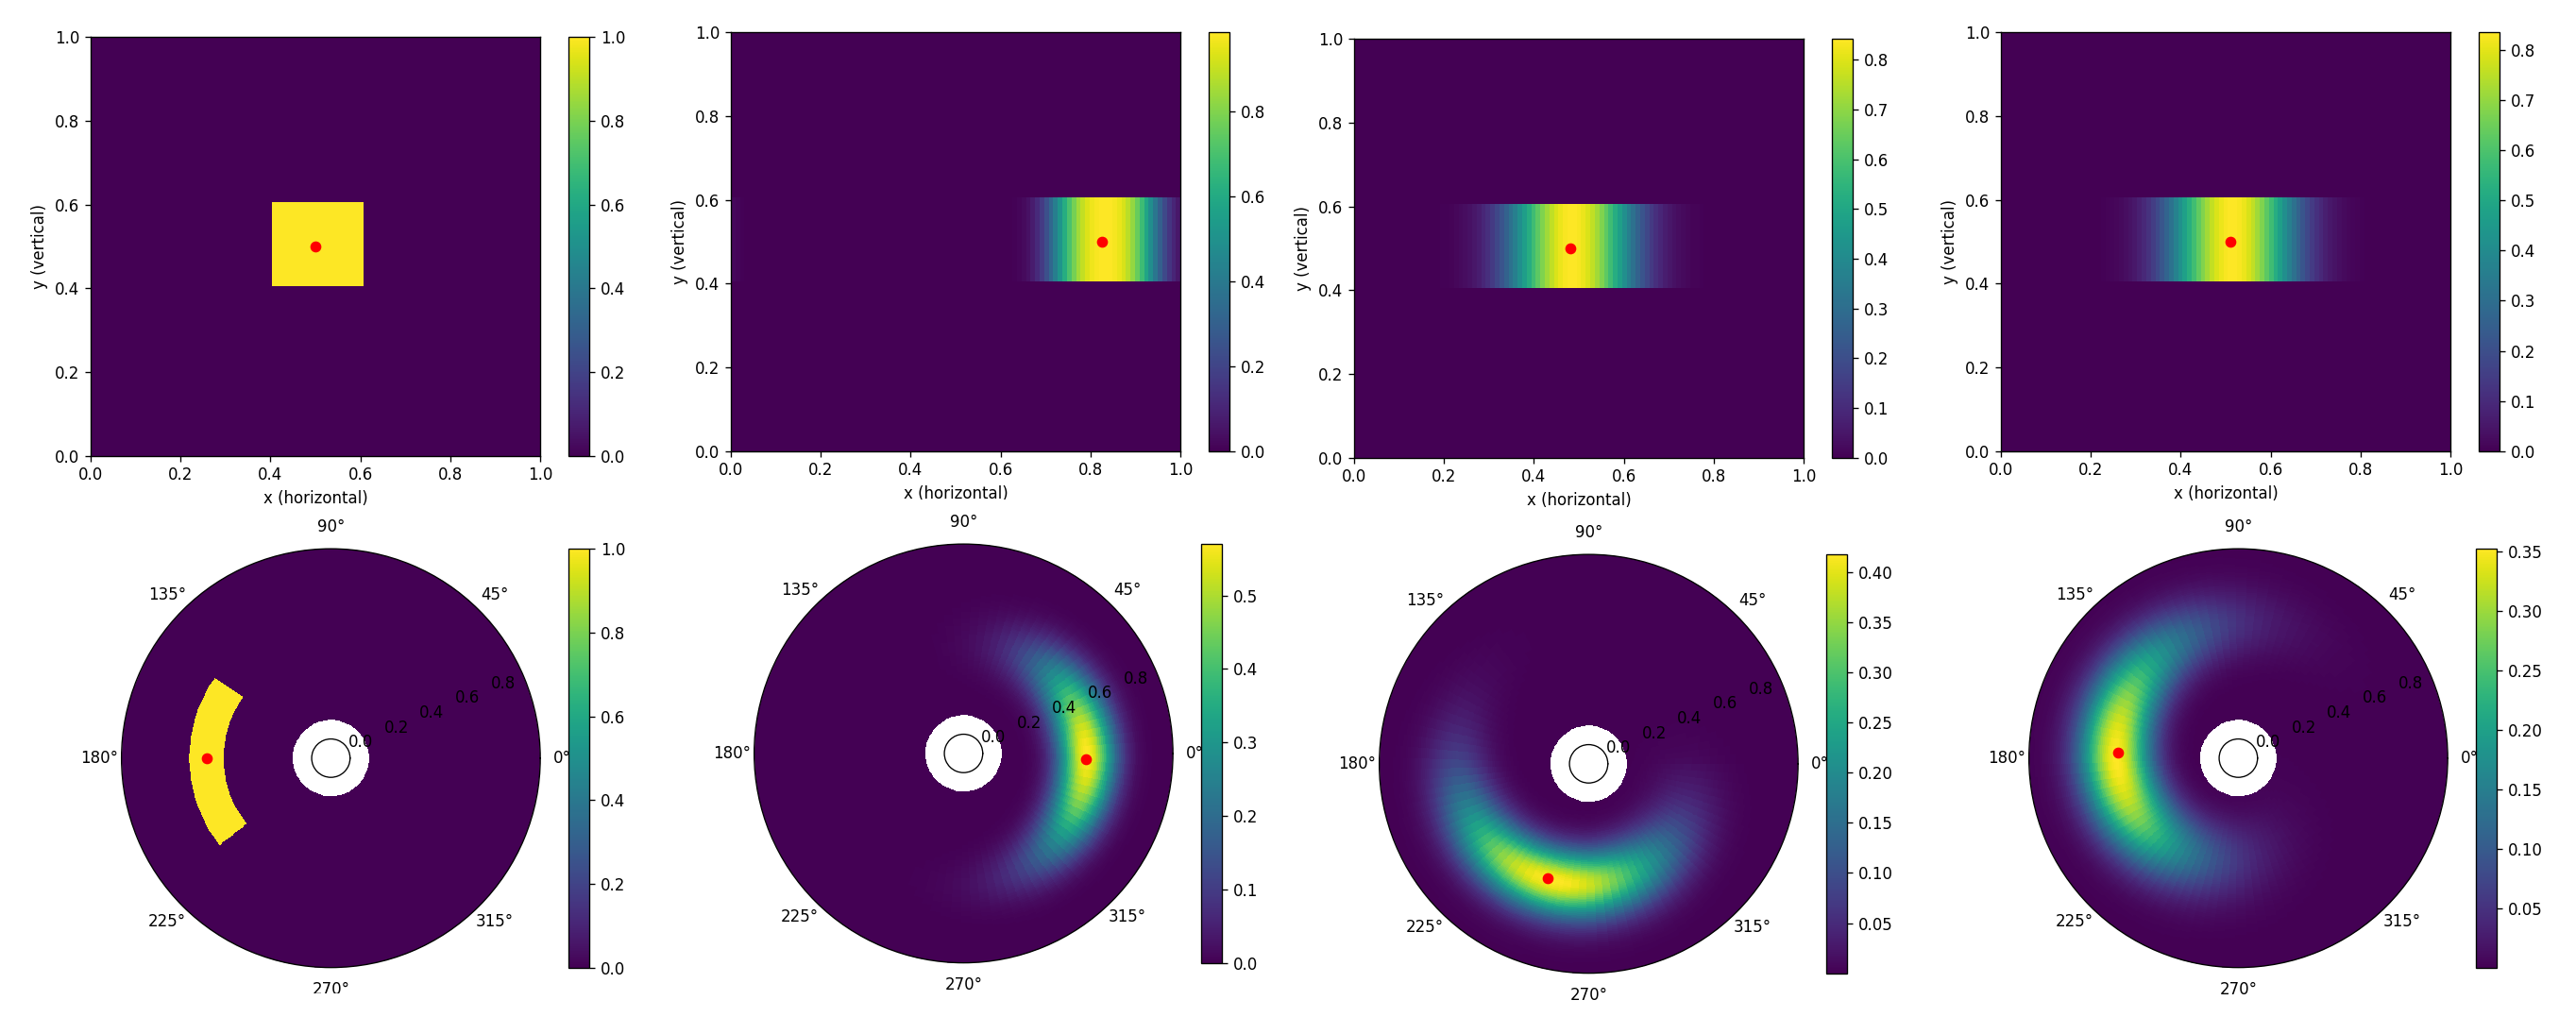
\includegraphics[scale=1.20]{combinedPeriodic.png}
	\caption{Cartesian (top) and polar (bottom) advection tests for horizontal (top) and azimuthal (bottom) advection. Advection fields move left to right (top) and clockwise (bottom). Red dot is centroid location, temperature indicated by colour. First column is the initial state, second column is crossing of periodic boundary conditions, third column is time when an exact scheme would return to the initial state, fourth column is advected field after returning to its initial location.}
	\label{periodic advection figure}
\end{sidewaysfigure}


\begin{sidewaysfigure}
	\center
	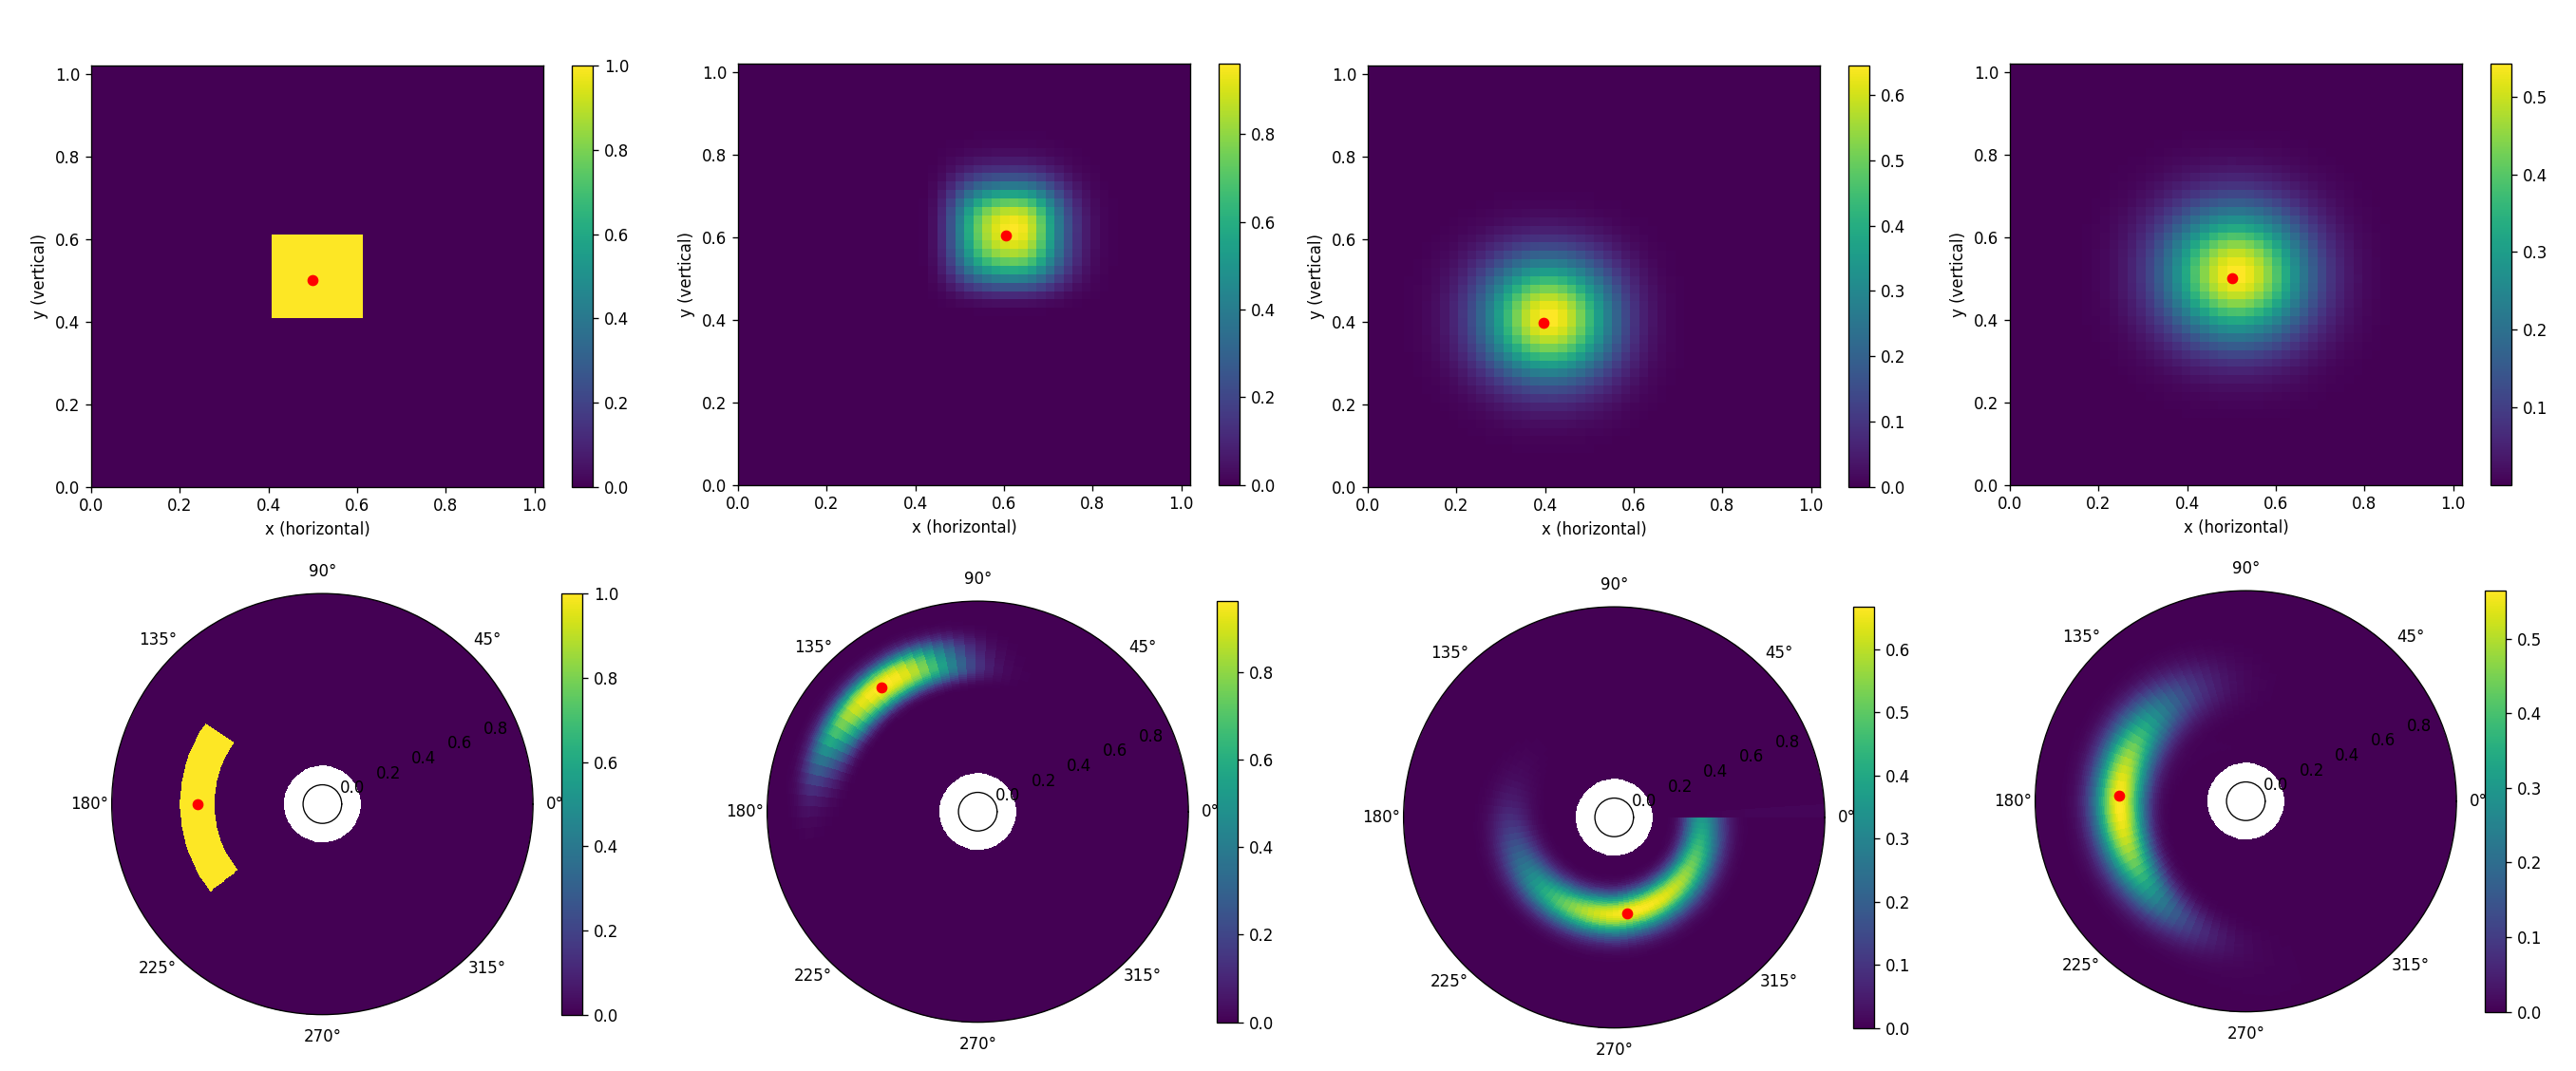
\includegraphics[scale=1.20]{combinedDiagonal.png}
	\caption{Cartesian (top) and polar (bottom) advection tests for advection back and forth along the secondary diagonal. Red dot is the centroid location, temperature indicated by colour. First column is the initial state, second column is one extreme of the diagonal, the third column is the other extreme and the final column is the state once the centroid has returned to its initial position.}
	\label{diagonal advection figure}
\end{sidewaysfigure}

\newpage
\section*{Advection tests}
{\it{A particularly difficult part of the streamfunction-vorticity simulation is correctly modelling advection. In this section, I perform some tests to show that my advection scheme works.}}
\vspace{0.3cm}
\newline
\noindent Thermal diffusivity ($\kappa$) and thermal expansion ($\alpha$) were set to zero to avoid convection. The fluid was set to temperature 0 (arb. units) except a small segment which was set to $1$ shown in yellow top left of figures \ref{periodic advection figure} and \ref{diagonal advection figure}. A streamfunction $\psi_c$ was enforced to produce diagonal back and forth motion or a continuous horizontal or azimuthal motion to cross a periodic boundary.




\noindent The advection results for both codes are similar. For the periodic advection test, top row figure \ref{periodic advection figure} and \ref{diagonal advection figure} the temperature 1 region is advected across the periodic boundary conditions without distortion. The centroid (red dot) lagged the advection field by $\approx 1 \%$ and $\approx 10 \%$ in the horizontal and azimuthal advection case (figure \ref{periodic advection figure}) respectively. It is unknown exactly why these differ substantially, however a probable cause is the smaller timestep use to produce the polar tests. In all cases, the blurring shows numerical diffusion along the direction of travel which is consistent with the modified equivalent partial differential equation for equation \ref{adeT} using our numerical scheme. The discontinuity in temperature in the bottom row third column of figure \ref{diagonal advection figure} near the $0, 360$ azimuthal angle boundary is a direct result of manually setting the streamfunction.

\section*{Thermal Lattice Boltzmann Tests}
To test the validity of my thermal lattice Boltzmann code, results from  \cite{mora2017simulation} are replicated in in figure \ref{Lattice Boltzmann 
Check}. I used a ''bounceback" boundary condition on all walls of the domain (figure \ref{Lattice Boltzmann Check} top four panes) which was compared 
against a simulation (figure \ref{Lattice Boltzmann Check} bottom) with the vertical walls having periodic boundary conditions. In addition, I used 
random fluctuations in boundary temperature of $10 \%$ while \cite{mora2017simulation} used random fluctuations of $25 \%$. The results are similar in 
convective plume size, quantity and definition. The convection begins slower in the simulation written here, but this can be accounted for by the smaller 
random noise used.


\begin{figure}[H]
	\centering
	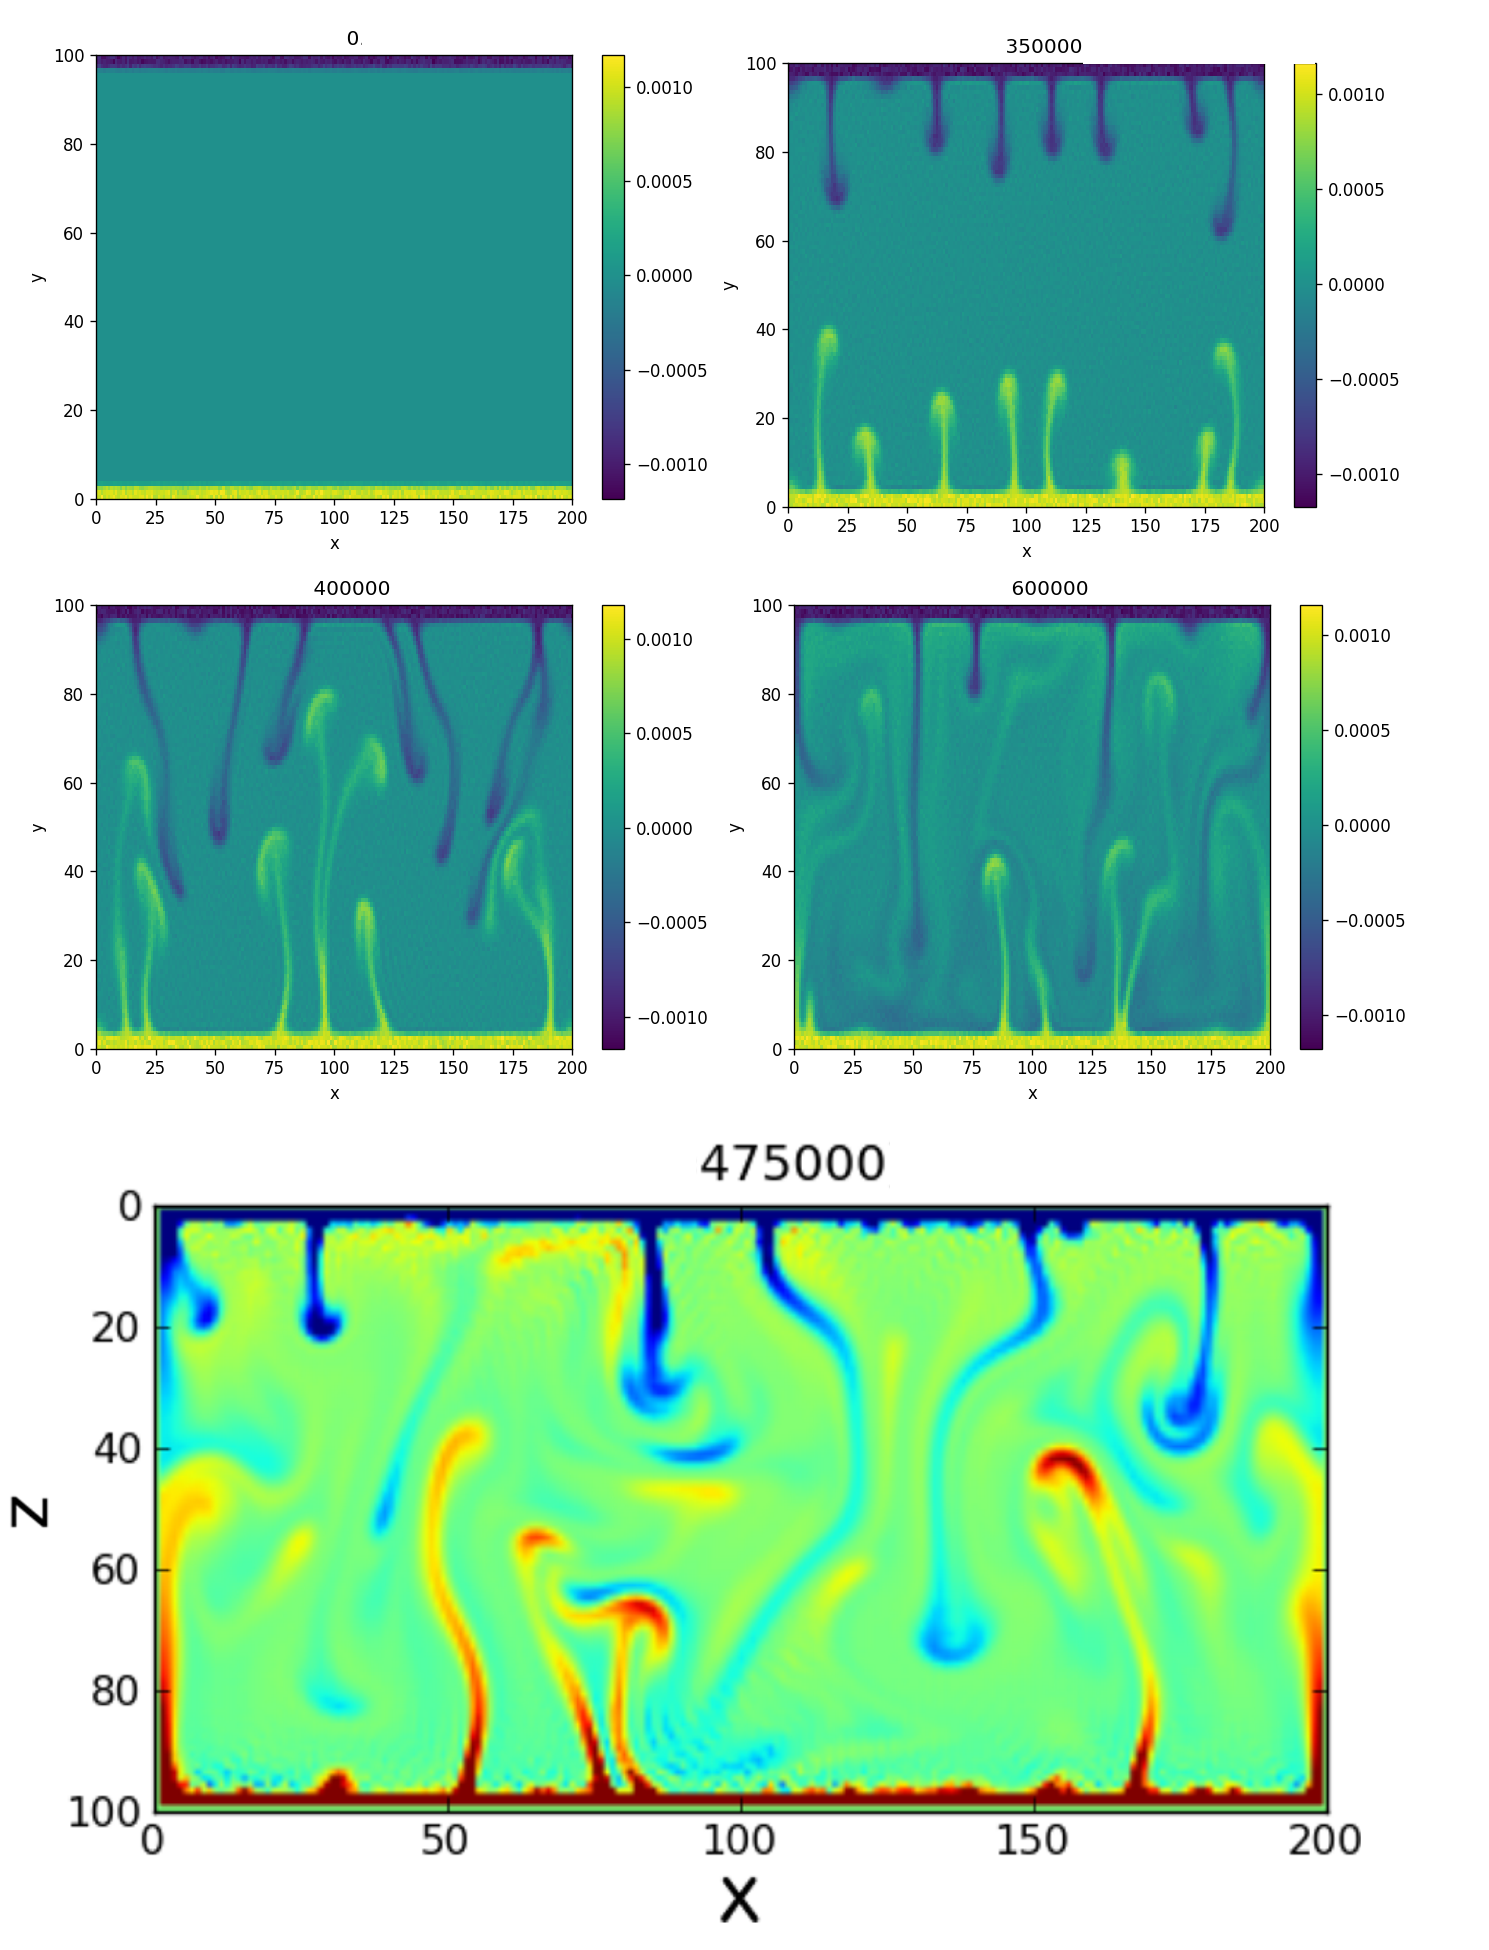
\includegraphics[scale=1.4]{latticeboltzmancheck.png}
	\caption{ Comparison between Thermal Lattice Boltzmann coded here (top four figures) and Published Thermal Lattice Boltzmann results (bottom figure) \cite{mora2017simulation}. Headings indicate timestep, red/yellow show hot regions while blue areas are cold. Top and bottom regions are held at constant temperature (no internal heating). All program settings used are similar. $Pr=5000, Ra=10^8$}
	\label{Lattice Boltzmann Check}
\end{figure}



\section*{Simulations}


\subsection*{Geometry and the Central region of a self-gravitating fluid}
{\it{In this section, I present results from my streamfunction-vorticity codes in Cartesian and polar coordinates. I show through comparison between simulations that taking into account the geometry and center of a 2-dimensional self gravitating fluid are important and significantly change both the dynamics and long term convective patterns.}}
\vspace{0.3cm}
\newline

\noindent A gravitational field linearly proportional to height and radius for the 
Cartesian and polar codes respectively was set. A constant internal 
heating field $H$ was set for all but the upper $10 \%$ of both domains. A 
compensating heating field was set at the remaining top of the domain to 
balance the total heat generation. Note this heat field is different in 
the Cartesian and polar cases. In all heating fields time-independent 
random fluctuations of $\approx 1 \%$ were set to facilitate instabilities.
\afterpage{%
\begin{figure}[H]
	\centering
	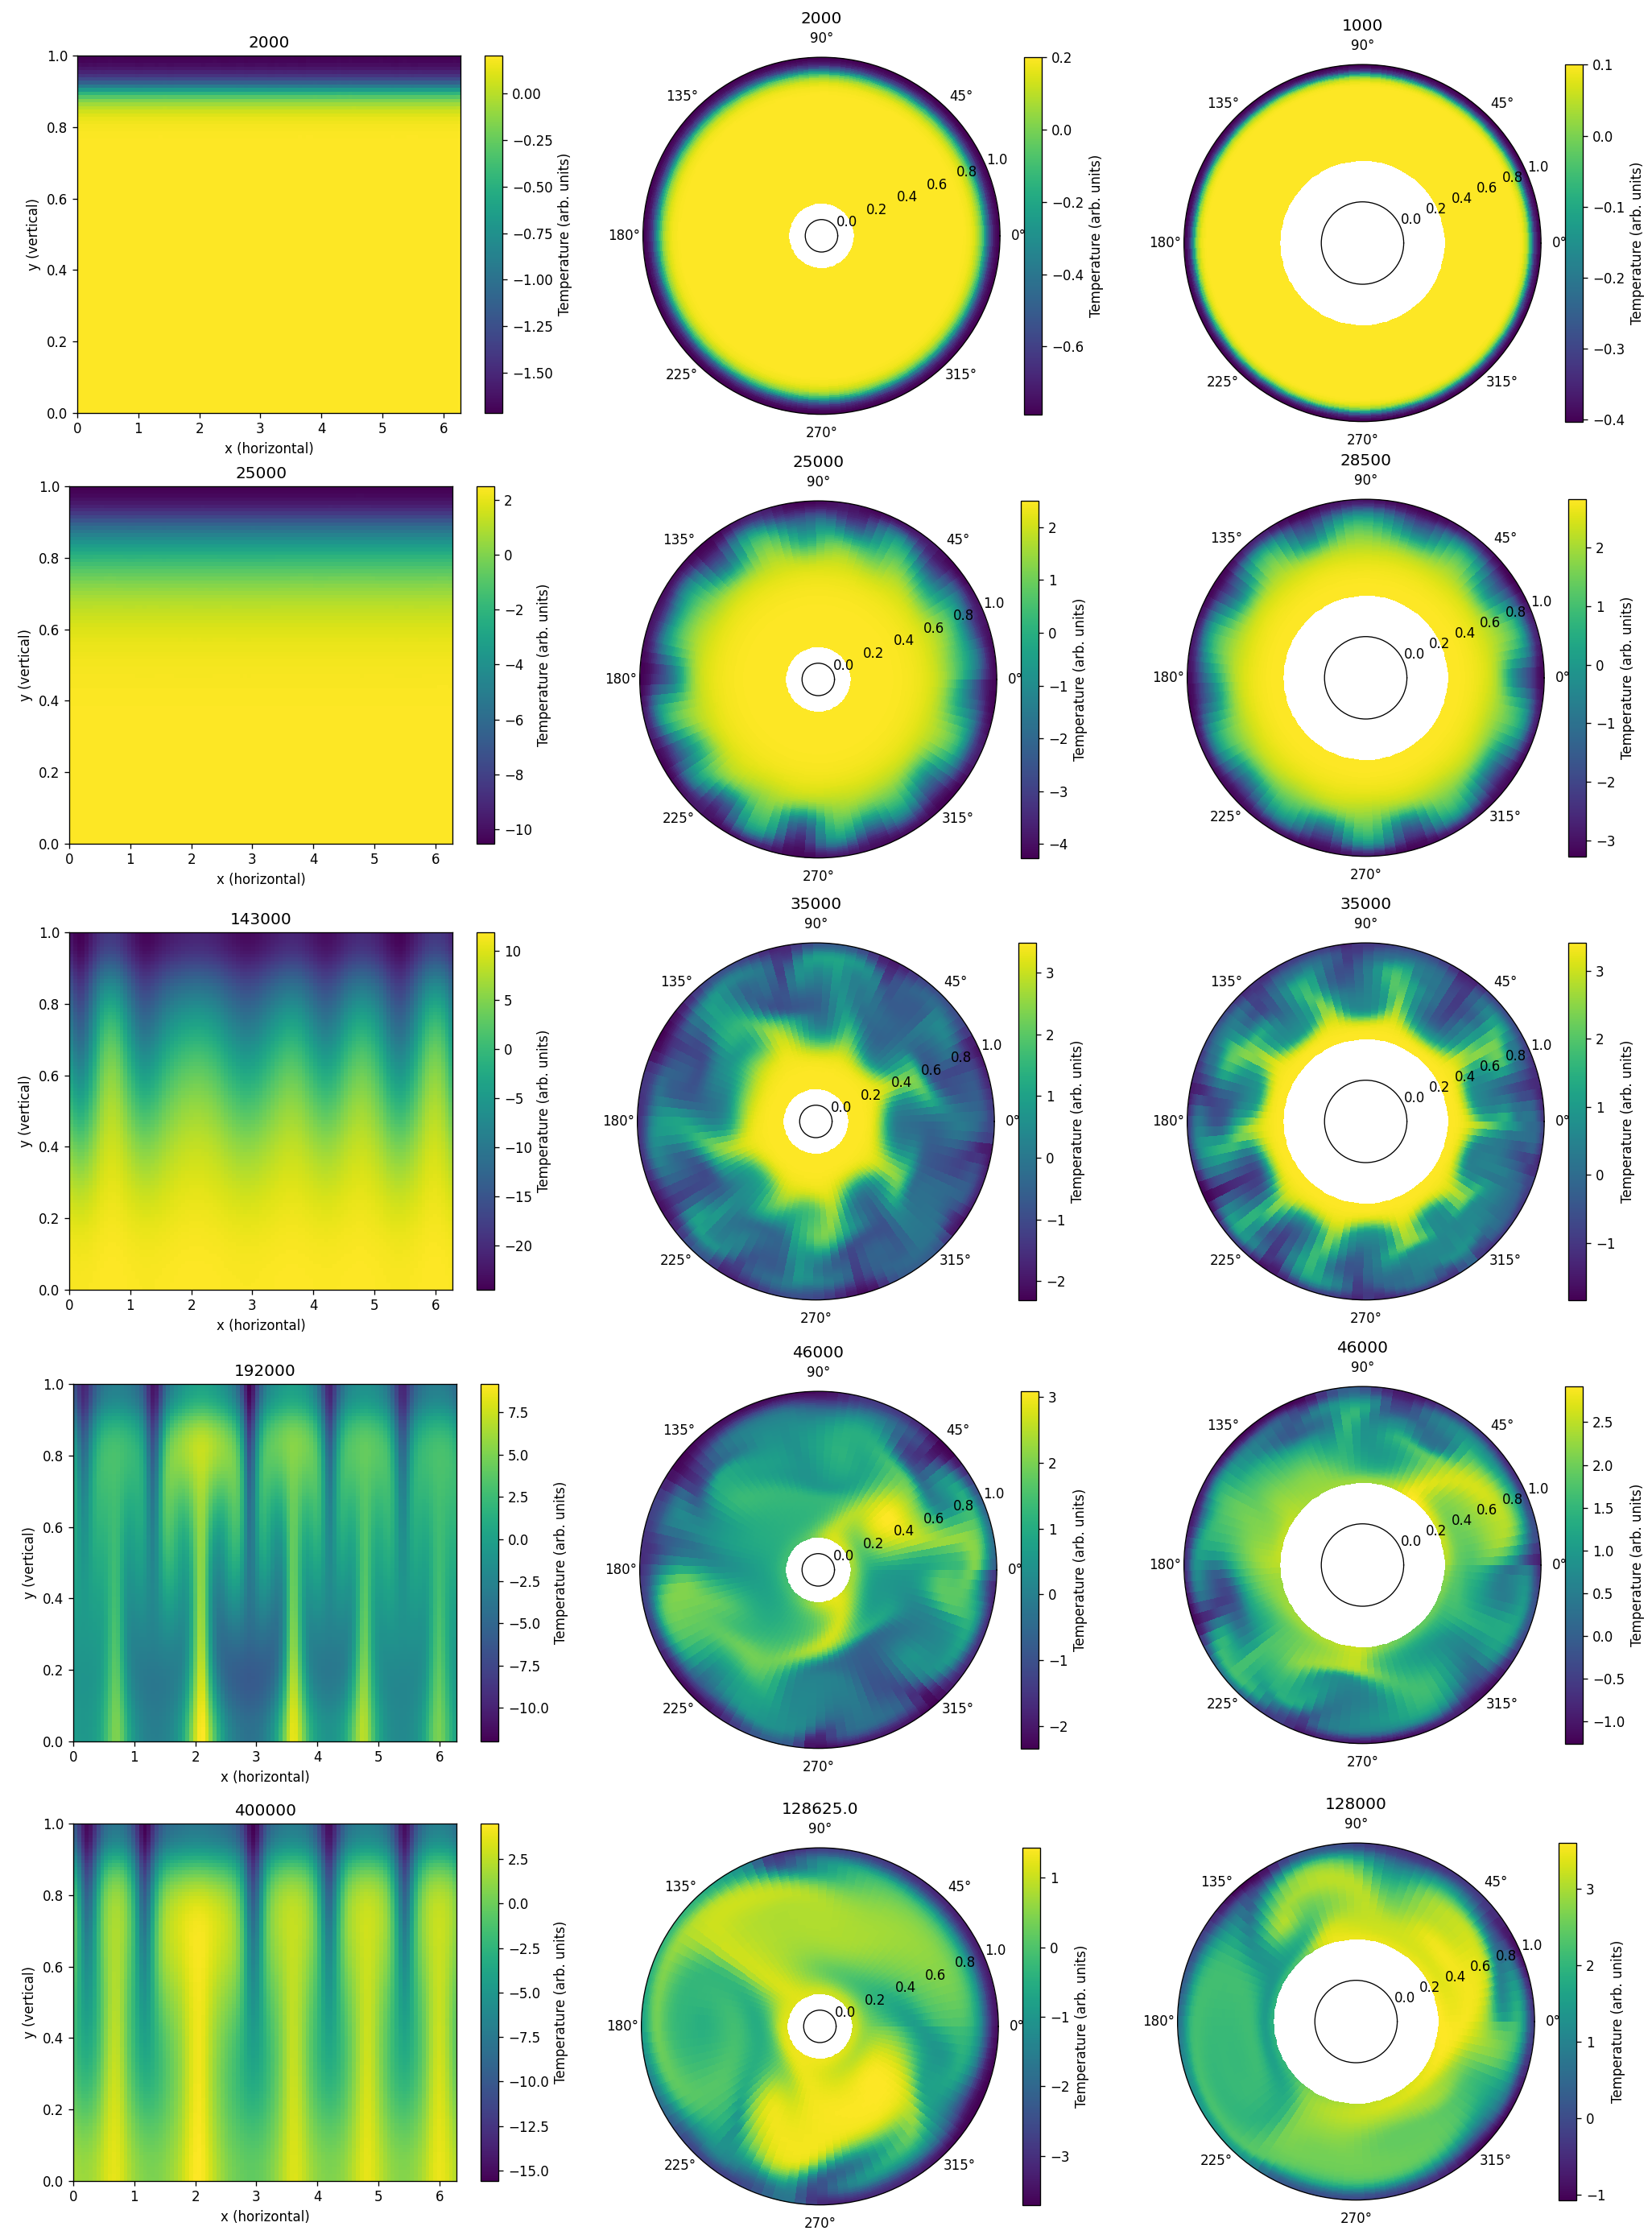
\includegraphics{streamfunctionComp.png}
	\caption{Simulations of internally heated, self-gravitating convection in Cartesian (left), polar with inner radius 0.1 (middle) and polar with inner radius 0.2 (right) coordinates. Times indicated by headings. Apart from inner radius, simulation settings are common. $Ra_H=10^8, Pr=5000$.}
	\label{cartesian vs polar}
\end{figure}
\clearpage
}

\noindent As seen in figure \ref{cartesian vs polar}, the two geometries give vastly different convective behaviour. The Cartesian geometry (left) begins forming 
convective plumes at time $\approx 143000$, long after the time $25000$ when the polar (middle) model begins to convect. The convection patterns formed 
in the Cartesian model are consistent in time, forming the typical Rayleigh-Bernard convection cells, while the polar cases are much more erratic. The larger inner radius polar simulation (right) shows similar initial behaviour to the smaller internal radius polar simulation (middle), however, it initially forms higher frequency convective structures. Importantly, over large timescales, the typical wavelength for features in the Cartesian geometry is $~3-5$ times longer. Therefore, in simulating a self-gravitating internally heated fluid such as the inner core accurately, the geometry and central region must be simulated. For traditional approaches which discretize a set of equations, this requires either complex spatial meshings or boundary conditions. 




\subsection*{Thermal Lattice Boltzmann Simulations}
{\it{In this section, I then present and discuss the results of my Thermal Lattice Boltzmann simulations. A video is available \href{https://www.youtube.com/watch?v=OM1oqFlu07A}{here} or via the url \url{https://www.youtube.com/watch?v=OM1oqFlu07A} to give the reader a better idea of the dynamics.}}
\vspace{0.3cm}
\newline
Figures \ref{LBM high Ra} and \ref{LBM low Ra} show TLBM simulations for internally heated Rayleigh 
numbers between $10^8$ and $10^4$ for Prandtl numbers of $Pr=5000$. A high Prandtl number was selected to show the applicability to geologic flows which operate in the larger Prandtl number limit. The heating field $H$ for these is constant below a radius of $90 \%$ and the 
remaining $10\%$ cooled so that the internal energy is constant. To stimulate convection, random fluctuations of $10 \%$ in the heating field were set as well as random fluctuations to the heating/cooling boundary. The initial state common to simulations in figures \ref{LBM high Ra} and \ref{LBM low Ra} is shown in figure \ref{LBM initial state}. 
\newline
%% then here I want to analyse these plots, what is happening here.
\noindent Figures \ref{LBM high Ra} and \ref{LBM low Ra} show that internally heated convection in our model begins at a thermal Rayleigh number below 
$Ra_H=10^5$. This lower bound is significantly higher than the critical Rayleigh number of $Ra\approx650$. However, these this critical Rayleigh number does not 
account for the polar geometry or non-constant gravitational field simulated here. The thermal Rayleigh number ($Ra_H$) is also related to the Rayleigh 
number ($Ra$) by scaling arguments and so is not directly comparable. We also do not know if the lack of convection in small thermal Rayleigh numbers 
like $Ra=10^4$ in figure \ref{LBM high Ra} is due to physical constraints, or the fact that we only simulated a finite amount of time. In future, the 
TLBM program could be parallelised (which is easy with goLang) and run for longer to simulate more steps and better bound the critical $Ra_H$ from above. The thickness of the cooling boundary layer used here is also not analysed, in future this could be done away with by using more complex thermal boundary conditions.  

%% Here I need to talk about the instabilities 
\noindent he characteristic wavelength of the convective patterns in figures \ref{LBM high Ra} and \ref{LBM low Ra} decreases with increasing thermal Rayleigh number ($Ra_H$). For small convecting thermal Rayleigh numbers, $Ra_H=10^6, Ra_H=10^5$ the convection wavelength is fairly consistent through time, while for higher values $Ra_H=10^8,Ra_H=10^7$ the wavelength is more dynamic. In general, the characteristic convection cells seen in Cartesian convection such as that in figure \ref{cartesian vs polar} (left bottom) is not seen. Instead, we see periodic plumes with skinny stalks and wide heads. These patterns are not static, best seen by the dumbbell-shaped oscillations in figure \ref{LBM low Ra} (left) indicating that these systems have not reached equilibrium. 

\begin{figure}[H]
	\centering
	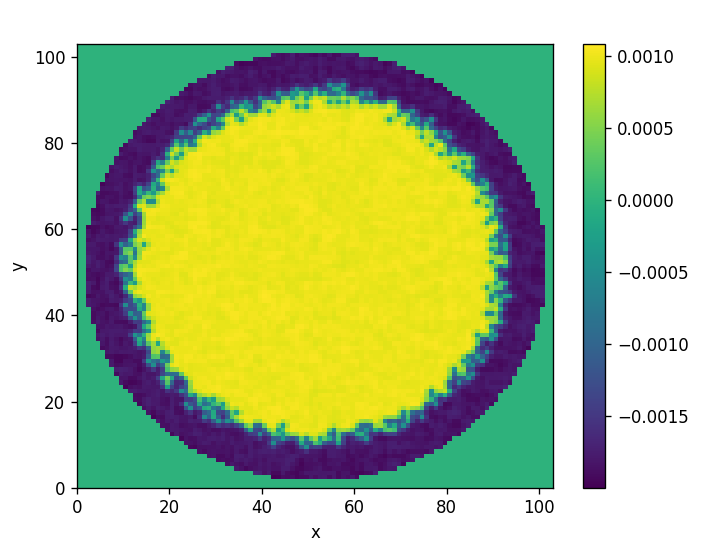
\includegraphics[scale=1.5]{initialState.png}
	\caption{Example Initial state showing random fluctuations of the heating field of $10 \%$ throughout with random fluctuations across the hot/cold boundary. }
	\label{LBM initial state}
\end{figure}

\afterpage{%
\begin{figure}[H]
	\centering
	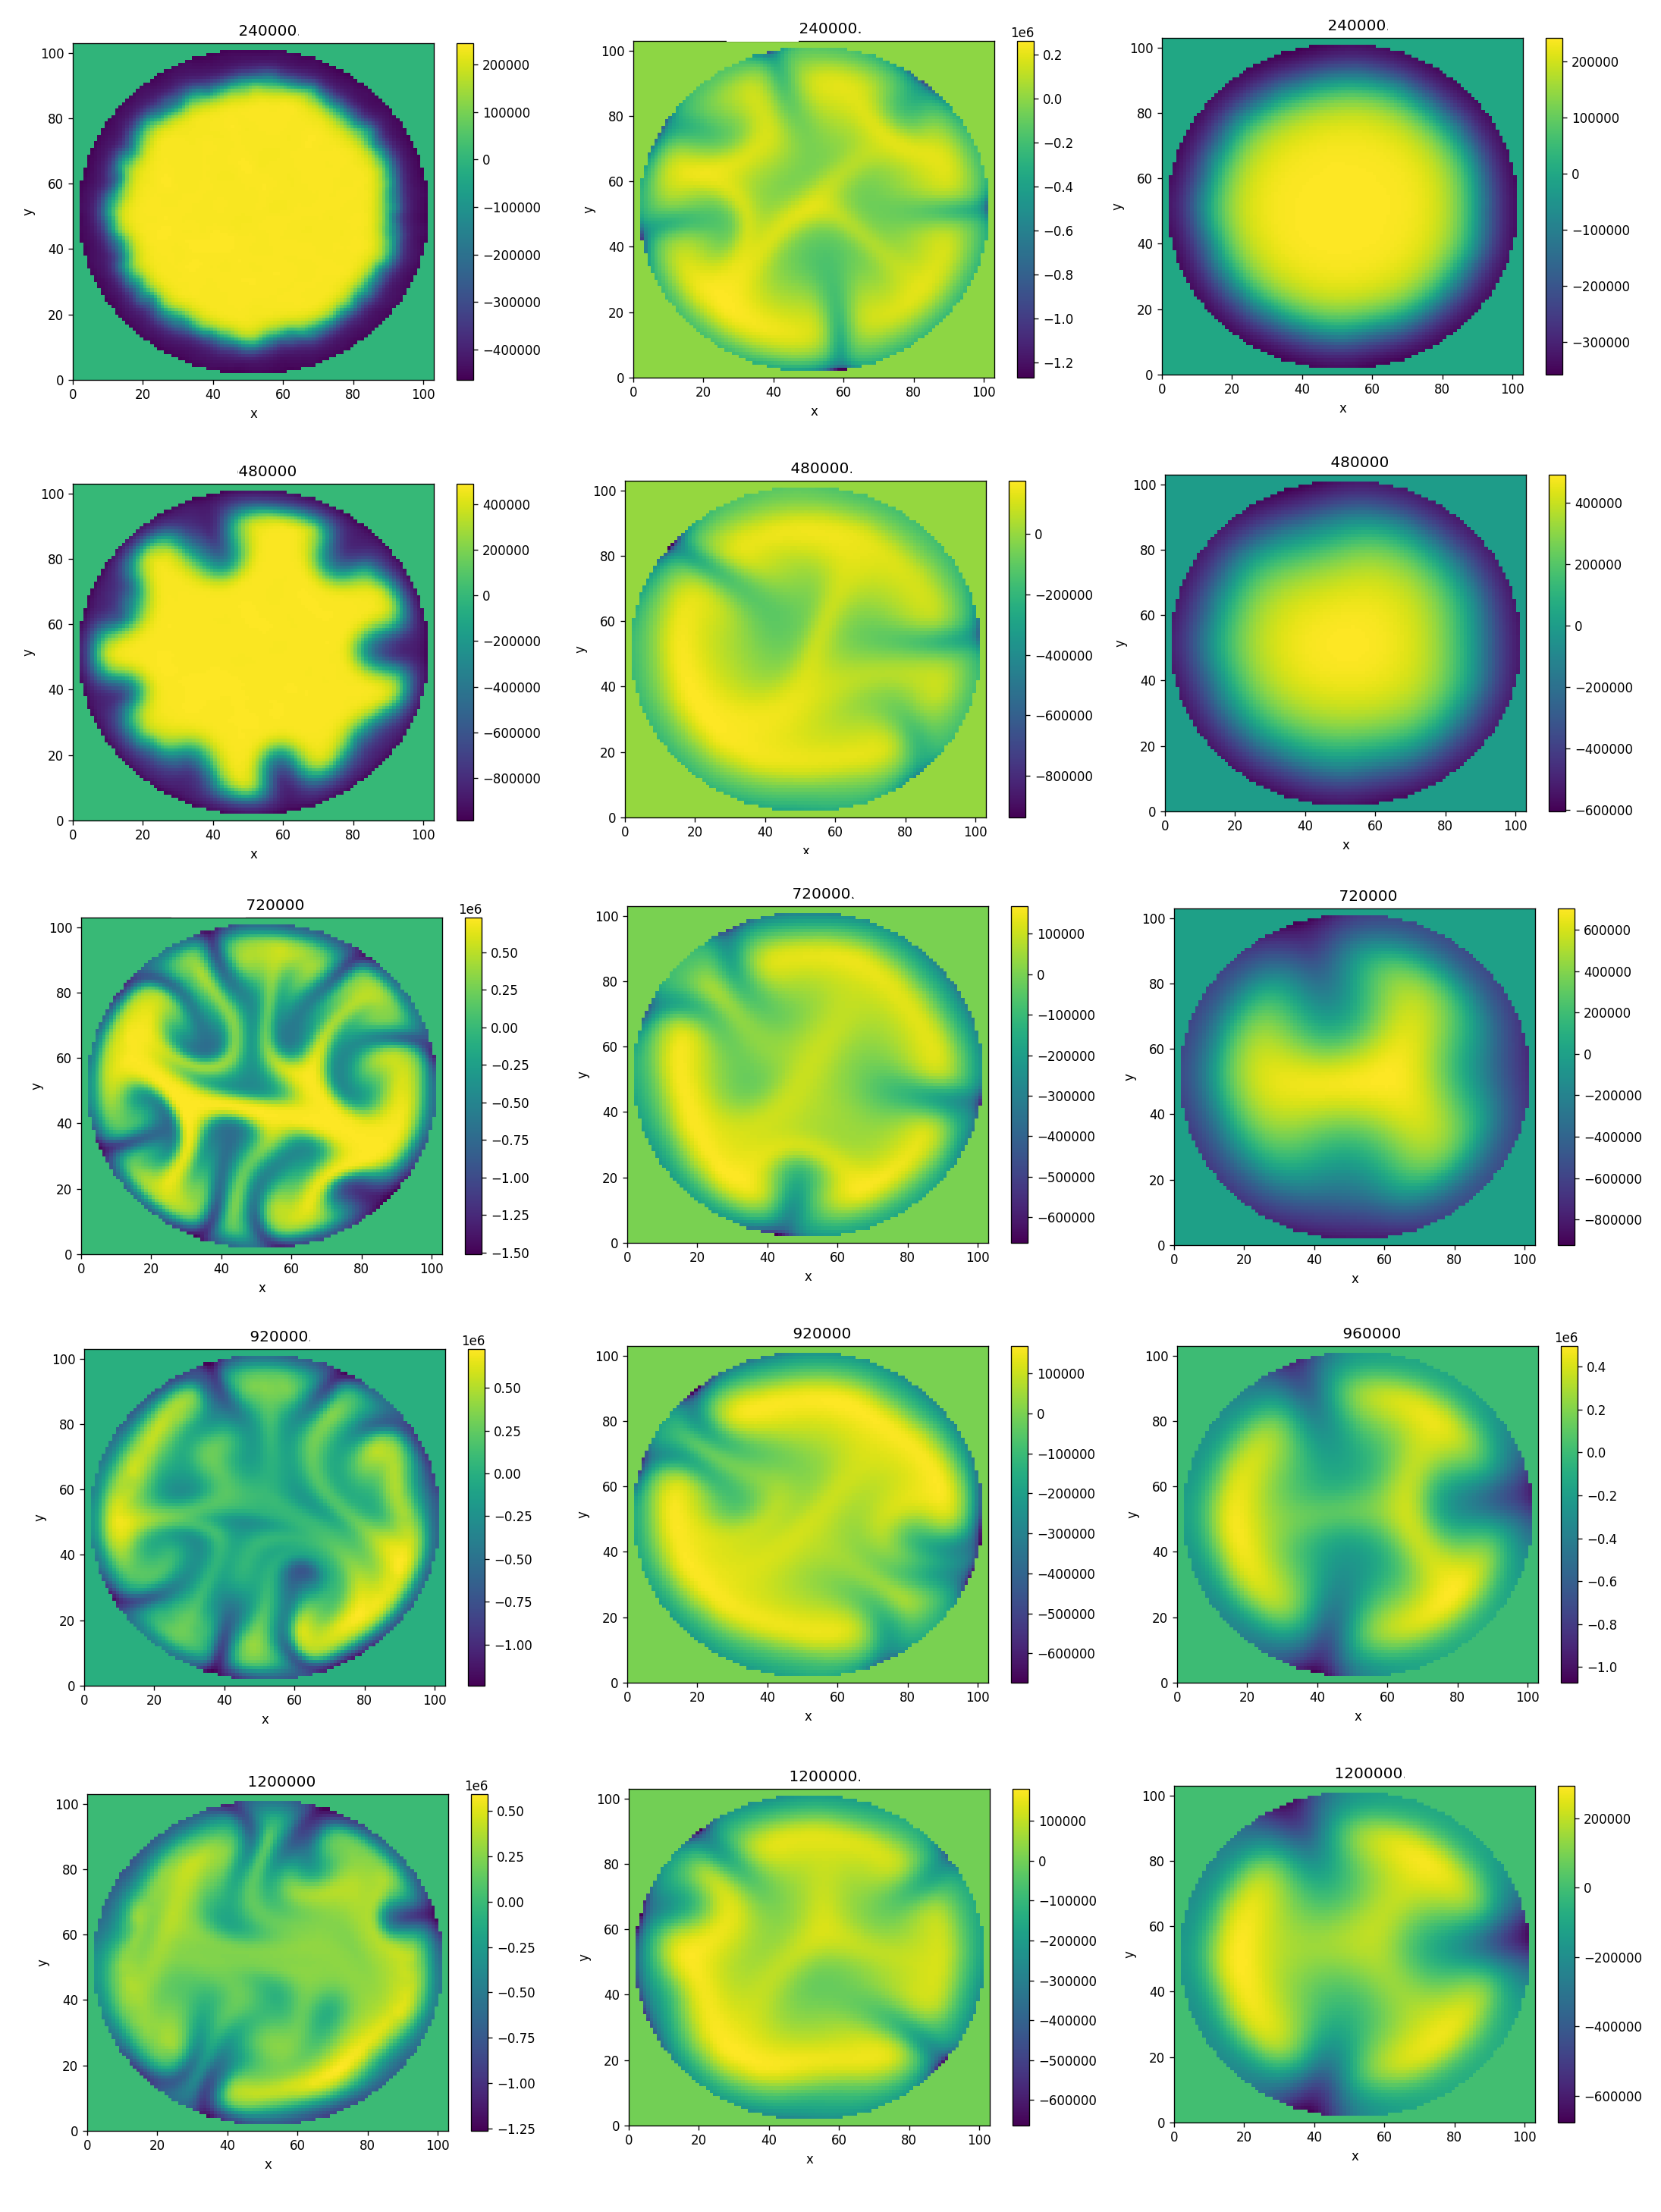
\includegraphics{latticeBoltzmanHighRa.png}
	\caption{High Rayleigh number $Ra_H=10^8$ (left column) $Ra_H=10^7$ (middle column) $Ra_H=10^6$ (right column) from Thermal Lattice Boltzmann simulations for an internally heated self-gravitating fluid with $Pr=5000$. Headings are simulation timestep}  
	\label{LBM high Ra}
\end{figure}
\clearpage
}

\afterpage{%
\begin{figure}[H]
	\centering
	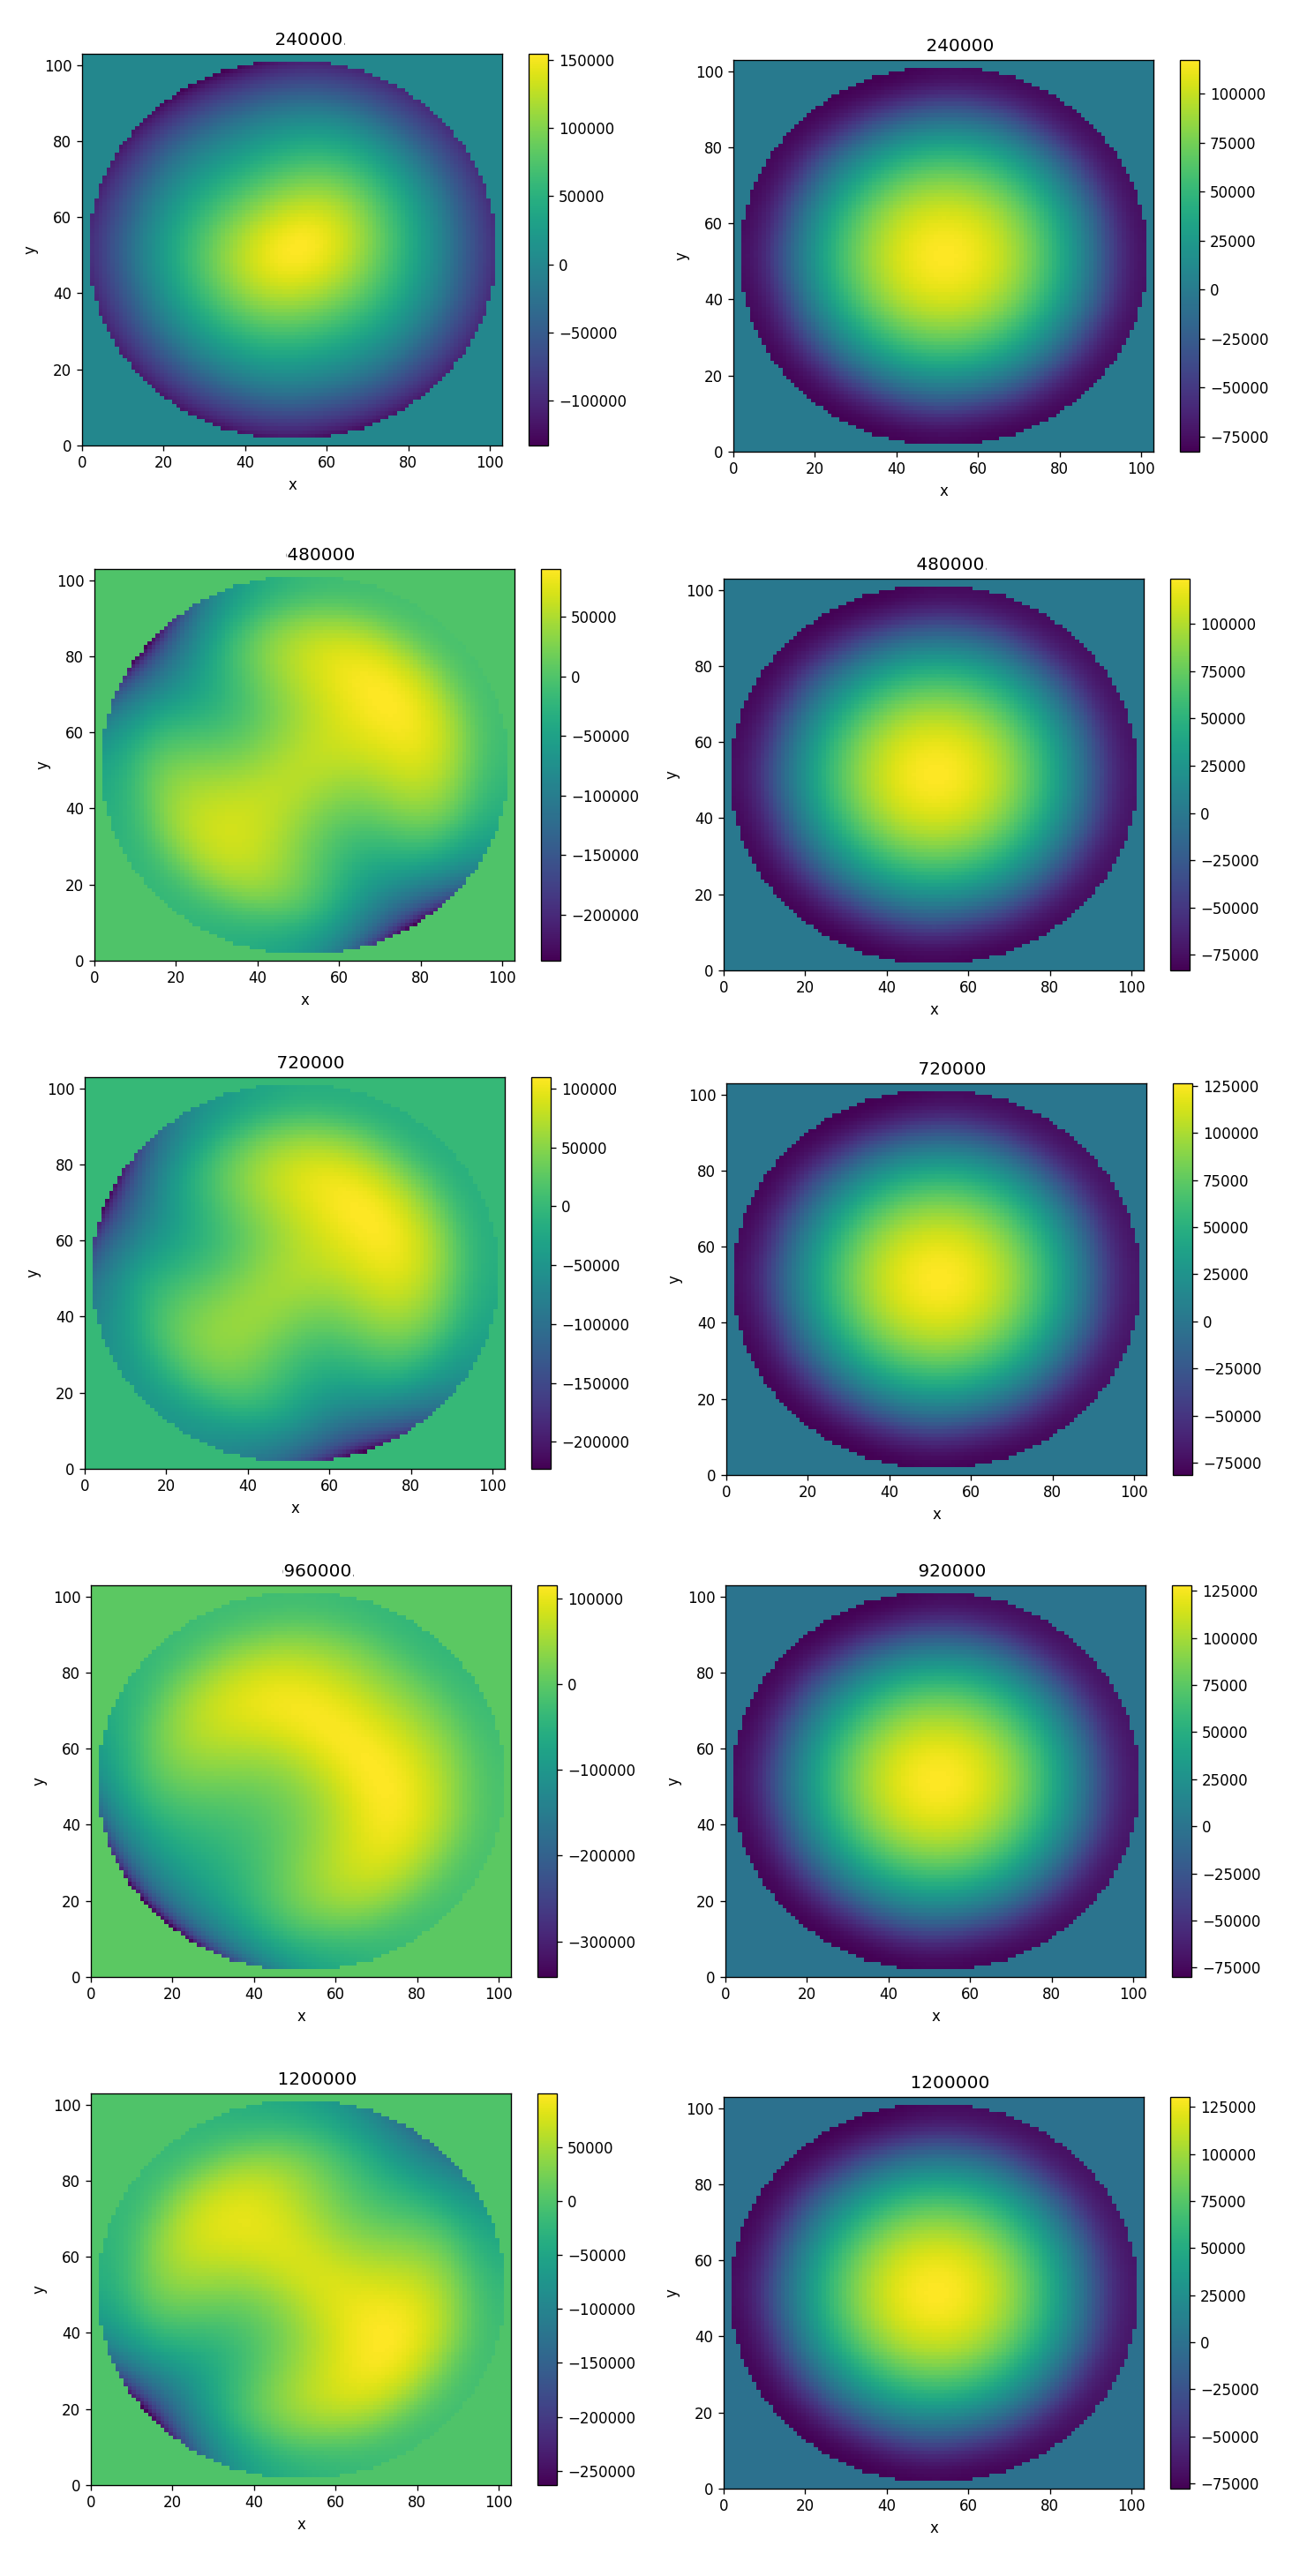
\includegraphics{latticeBoltzmanLowRa.png}
	\caption{High Rayleigh number $Ra_H=10^5$ (left column) $Ra_H=10^4$ (right column) Thermal Lattice Boltzmann simulations for an internally heated self-gravitating fluid with $Pr=5000$. Headings are simulation timestep}  
	\label{LBM low Ra}
\end{figure}
\clearpage
}



\subsection*{Difficulties with the Thermal Lattice Boltzmann method}
The TLBM coded here uses a fixed unit timestep and lattice spacing making the lattice speed $C=1$. The TLBM remains stable as long as the macroscopic velocities remain a small fraction of the lattice speed. For internally heated convective problems, the time to heat/cool the fluid before convective plumes can develop can be significant compared to the timescale for plume motion, particularly at smaller or near critical Rayleigh numbers. Because of this, much simulation time is spent computing an uninteresting part of the solution. 
\newline
\noindent Extreme local heating or cooling was also an issue that would occur at high Rayleigh numbers $Ra>10^9$ and induce velocities comparable to the lattice speed, causing instabilities to grow to infinity and crash the program.
\newline



\section*{Conclusion}
%% need to rewrite this.

A 2-dimensional self-gravitating internally heated model of the inner core was presented. Codes 
were developed from scratch in python3 and goLang to simulate convection in the model using 
streamfunction-vorticity and Lattice Boltzmann approaches. The streamfunction codes based in 
Cartesian and polar geometries were compared showing that the geometry and central region of the 
inner core were important to accurately simulating internally heated convection, however neither 
code could account for both. Finally, results from the TLBM code which accounted for both geometry 
and the central region were presented for high Prandtl number ($Pr=5000$) giving an upper bound on 
the critical internally heated Rayleigh number of $Ra_H < 10^5$. In future, the same Lattice Boltzmann
code could be used to model more realistic models of the inner core, which involve other heat sources such as surface heating from 
friction or heat left over from Earth's formation. It can also be applied to other problems with otherwise difficult non-slip
boundary conditions.




\newpage
\section*{Appendix}
	\subsection*{The Jacobi Method}
	{\it{Here the Jacobi Method for solving the Poisson equation, like (\ref{psi}) is introduced. This is the method used for solving \ref{psi} used in my streamfunction-vorticity codes.}}
	\vspace{0.3cm}
	\newline
	We cannot solve for $\psi$ explicitly in equation \ref{psi}. Instead we use an iterative Jacobi method. In Cartesian coordinates, equation \ref{psi} is:
	\begin{equation}
		\omega_{i,j} = \frac{\psi_{i+1,j} - 2 \psi_{i,j} + \psi_{i-1,j}  }{{\Delta x}^2} + \frac{\psi_{i,j+1} - 2 \psi_{i,j} + \psi_{i,j-1}  }{{\Delta y}^2}
		\label{psi disc}
	\end{equation}
	Rearranging for $\psi$
	\begin{equation}
		\psi_{i,j} = \frac{{\Delta x}^2 {\Delta y}^2  }{2({\Delta x}^2  + {\Delta y}^2)} (\frac{\psi_{i+1,j} +\psi_{i-1,j} }{{\Delta x}^2} + \frac{\psi_{i,j+1} +\psi_{i,j-1}  }{{\Delta y}^2 }  + \omega_{i,j}).
		\label{psi from omega}
	\end{equation}
	We then use the result of $\psi_{i,j}$ back into equation \ref{psi from omega} to solve for $\psi_{i,j}$ iterately as shown in equation \ref{psi iterative} \cite{burkardt2011jacobi, adair2015developing}:
	\begin{equation}
		\psi_{i,j}^{(k+1)} = \frac{{\Delta x}^2 {\Delta y}^2  }{2({\Delta x}^2  + {\Delta y}^2)} (\frac{\psi_{i+1,j}^{(k)} +\psi_{i-1,j}^{(k)}  }{{\Delta x}^2} + \frac{\psi_{i,j+1}^{(k)} +\psi_{i,j-1}^{(k)}  }{{\Delta y}^2 } + \omega_{i,j}).
		\label{psi iterative}
	\end{equation}
	Where the superscript $(k)$ means the result of the $k^{th}$ iteration of the above equation and this operation us applied to all points in $\mathcal{D}'$.
	 We terminate this iterative method once the error $\sum_{(i,j) \in \mathcal{D'}} \mid \psi_{i,j}^{(k+1)} - \psi_{i,j}^{(k)} \mid$ gets sufficiently small. A similar method is applied in polar coordinates. 

\bibliographystyle{abbrv}
\bibliography{ref.bib}





\end{document}
